\documentclass[12pt, a4paper]{article}

% ─── Packages ────────────────────────────────────────────────────────────────
\usepackage{lmodern}
\usepackage{amssymb}
\usepackage[utf8]{inputenc}
\usepackage[T1]{fontenc}
\usepackage[italian]{babel}
\usepackage{geometry}
\geometry{margin=2.5cm}
\usepackage{microtype}
\usepackage{parskip}
\usepackage{setspace}
\setstretch{1.15}

\usepackage{graphicx}
\usepackage{hyperref}
\hypersetup{
    colorlinks=true,
    linkcolor={blue!60!black},
    urlcolor={blue!60!black},
    citecolor={blue!60!black}
}
\usepackage{listings}
\usepackage{xcolor}
\usepackage{booktabs}
\usepackage{float}
\usepackage{array}
\usepackage{enumitem}
\usepackage{fancyhdr}
\usepackage{titlesec}
\usepackage{tikz}
\usetikzlibrary{positioning, arrows.meta, calc, fit}

% ─── Stile codice ────────────────────────────────────────────────────────────
\lstset{
    basicstyle=\ttfamily\small,
    keywordstyle=\color{blue!70!black}\bfseries,
    commentstyle=\color{gray!70}\itshape,
    stringstyle=\color{orange!80!black},
    breaklines=true,
    breakatwhitespace=true,
    frame=single,
    rulecolor=\color{gray!40},
    backgroundcolor=\color{gray!8},
    numbers=left,
    numberstyle=\tiny\color{gray},
    captionpos=b,
    tabsize=4,
    showstringspaces=false,
    postbreak=\mbox{\textcolor{gray}{$\hookrightarrow$}\space}
}

% ─── Header / Footer ─────────────────────────────────────────────────────────
\pagestyle{fancy}
\fancyhf{}
\rhead{SW Engineering for Secure Cloud Systems}
\lhead{\leftmark}
\cfoot{\thepage}

% ─── Macro UML ───────────────────────────────────────────────────────────────
% \umlclass{id}{x}{y}{Titolo}{Attributi}{Metodi}{fill-color}{draw-color}
\newcommand{\umlclass}[8]{%
    \node[
        draw=#8, fill=#7, thick,
        minimum width=3.8cm, minimum height=0.65cm,
        font=\small\bfseries\ttfamily, text=black, anchor=north
    ] (#1-title) at (#2,#3) {#4};
    \node[
        draw=#8, fill=#7!30, thick,
        minimum width=3.8cm,
        font=\small\ttfamily, text=black,
        align=left, inner sep=4pt, anchor=north
    ] (#1-attr) at (#1-title.south) {#5};
    \node[
        draw=#8, fill=#7!20, thick,
        minimum width=3.8cm,
        font=\small\ttfamily, text=black,
        align=left, inner sep=4pt, anchor=north
    ] (#1-meth) at (#1-attr.south) {#6};
}

% ─── Titolo ──────────────────────────────────────────────────────────────────
% ─── Titolo ──────────────────────────────────────────────────────────────────
\title{
    \vspace{-1cm}
    
\includegraphics[width=4cm]{logo_unisa.png}\\[1cm]
    \Large \textbf{Universit\`a degli Studi di Salerno}\\
    \large Corso di Laurea Magistrale in
    Sicurezza Informatica e Tecnologie Cloud (LM-66)\\[0.5cm]
    \rule{\textwidth}{0.4pt}\\[0.4cm]
    {\LARGE \textbf{Rent a Car Backend}}\\
    {\large Progetto di SW Engineering for Secure Cloud Systems}\\
    \rule{\textwidth}{0.4pt}
}
\author{
    Andrea Aselli \quad Benedetto Pio Turino \quad Emanuele Pascale\\[0.5cm]
    \small Universit\`a degli Studi di Salerno
}

\date{Anno Accademico 2025/2026}
% ─────────────────────────────────────────────────────────────────────────────
\begin{document}

    \maketitle
    \thispagestyle{empty}
    \newpage

    \tableofcontents
    \newpage

% =============================================================================
    \section{Scopo del Progetto}

    L'obiettivo di questo progetto è analizzare e mettere in sicurezza
    \textbf{ExtendRent}, un'applicazione backend per la gestione del noleggio di
    autoveicoli sviluppata con \textbf{Spring Boot}, seguendo i principi del
    \emph{Secure Software Development Lifecycle} (SSDLC).

    Il lavoro si articola nelle seguenti fasi principali:
    \begin{enumerate}
        \item \textbf{Analisi dell'architettura}: studio del sistema, dello stack
        tecnologico e delle superfici di attacco.
        \item \textbf{Identificazione delle vulnerabilità}: analisi statica manuale del
        codice sorgente; identificazione di 15 vulnerabilità classificate per
        severità e categoria.
        \item \textbf{Mitigazione}: applicazione di patch mirate per risolvere tutte le
        vulnerabilità identificate.
        \item \textbf{Verifica tramite test}: scrittura di una suite di test di sicurezza
        a copertura delle vulnerabilità patchate, con esito 100\% pass.
        \item \textbf{Containerizzazione}: packaging dell'applicazione con Docker,
        adottando pratiche di sicurezza nella configurazione dei container.
    \end{enumerate}
% =============================================================================
    \section{Descrizione dell'Applicazione}
% =============================================================================

    \textbf{ExtendRent} è un sistema di gestione
    per il noleggio di autoveicoli sviluppato come backend REST API, disponibile
    pubblicamente su GitHub al seguente indirizzo:
    \begin{center}
        \url{https://github.com/aaselli2-unisa/rentACar_backend/tree/master}
    \end{center}

    \noindent{ExtendRent} risolve il problema della gestione completa del ciclo di
    vita di un noleggio: dalla registrazione del cliente alla selezione del
    veicolo, dalla creazione del contratto al pagamento, fino alla restituzione
    del mezzo.

    \subsection*{A chi è destinato}

    \begin{table}[H]
        \centering
        \begin{tabular}{ll}
            \toprule
            \textbf{Ruolo} & \textbf{Utilizzo principale} \\
            \midrule
            Amministratori & Gestione completa del sistema: veicoli, utenti,
            sconti, report finanziari \\
            \midrule
            Dipendenti     & Gestione operativa dei noleggi, aggiornamento stato
            veicoli \\
            \midrule
            Clienti        & Ricerca veicoli disponibili, prenotazione e gestione
            dei propri noleggi \\
            \bottomrule
        \end{tabular}
        \caption{Ruoli e utilizzo principale del sistema ExtendRent.}
        \label{tab:ruoli}
    \end{table}

    \subsection*{Cosa fa}

    L'applicazione offre un sistema di autenticazione e autorizzazione basato su
    \textbf{JWT} con tre livelli di ruolo distinti: \emph{Admin}, \emph{Employee}
    e \emph{Customer}. Il catalogo veicoli è gestito con supporto a filtri avanzati
    su 23 attributi, mentre l'intero ciclo di vita del noleggio — dalla creazione,
    all'avvio, alla restituzione fino alla cancellazione — è tracciato e gestito
    dalla piattaforma. Sul fronte economico, il sistema elabora i pagamenti e
    produce reportistica dei ricavi mensili, annuali e totali, con supporto a
    codici sconto con percentuali configurabili. Le immagini di veicoli, utenti e
    brand vengono caricate su \textbf{Cloudinary}, mentre la verifica degli account
    avviene tramite email e OTP. Tutte le entità adottano il meccanismo di
    \emph{soft delete}, garantendo la cancellazione logica dei dati senza perdita
    di informazioni storiche. L'intera API è documentata tramite
    \textbf{Swagger~/ OpenAPI}.

    \subsection{Architettura e Funzionamento}

    L'applicazione segue un'architettura MVC:

    \begin{itemize}
        \item \textbf{Controller Layer} -- gestisce le richieste HTTP REST.
        \item \textbf{Service Layer} -- contiene la business logic.
        \item \textbf{Repository Layer} -- accesso ai dati tramite JPA/Hibernate.
        \item \textbf{Security Layer} -- autenticazione e autorizzazione JWT.
    \end{itemize}

    La sicurezza è gestita tramite \textbf{Spring Security}, con un filtro JWT
    (\texttt{JwtAuthFilter}) che intercetta ogni richiesta e valida il token.

    L'applicazione utilizza \textbf{PostgreSQL} come database relazionale e
    integra servizi esterni come:
    \begin{itemize}
        \item \textbf{Cloudinary} per la gestione delle immagini.
        \item \textbf{SMTP} per l'invio di email e OTP.
    \end{itemize}

    \subsection{Struttura del Progetto}

    Il progetto segue una struttura a stratiorganizzata per dominio funzionale:

    \begin{itemize}
        \item \textbf{\texttt{controller/}} -- Layer REST che riceve le richieste
        HTTP. Suddiviso per dominio: autenticazione (\texttt{auth/}),
        utenti (\texttt{user/}), veicoli (\texttt{vehicle/}), noleggi
        (\texttt{rental/}), pagamenti (\texttt{payment/}), sconti
        (\texttt{discount/}), patenti (\texttt{license/}) e immagini
        (\texttt{image/}).
        \item \textbf{\texttt{service/}} -- Layer di business logic, anch'esso
        suddiviso per dominio. Include servizi trasversali come
        \texttt{JwtService}, \texttt{EmailService} e \texttt{OtpService},
        oltre a un sottopacchetto \texttt{businessrules/} dedicato alle
        regole di validazione di dominio.
        \item \textbf{\texttt{repository/}} -- Layer di accesso ai dati tramite
        interfacce JPA. Comprende 23 repository, tra cui
        \texttt{CarRepository} con query custom per i filtri avanzati.
        \item \textbf{\texttt{core/}} -- Infrastruttura trasversale: configurazione
        della sicurezza (\texttt{SecurityConfig.java}), filtro JWT
        (\texttt{JwtAuthFilter.java}), seed dei dati iniziali
        (\texttt{SeedDataConfig.java}), gestione delle eccezioni custom e
        utilities AOP.
        \item \textbf{\texttt{Application.java}} -- Entry point Spring Boot,
        responsabile dell'avvio dell'applicazione, del seed dei dati e
        della visualizzazione del banner ASCII.
        \item \textbf{\texttt{pom.xml}} -- Descrittore Maven con tutte le
        dipendenze del progetto.
        \item \textbf{\texttt{application.properties}} -- Configurazione di
        database, JWT, server SMTP e Cloudinary.
    \end{itemize}

    \begin{lstlisting}[language=bash, caption={Struttura delle directory del progetto}]
rentACar_backend/
|-- pom.xml                      # Dipendenze Maven
|-- src/main/
    |-- java/src/
    |   |-- Application.java     # Entry point + seed dati
    |   |-- controller/          # Layer REST
    |   |   |-- auth/         # SignUp, SignIn, refresh token, OTP
    |   |   |-- user/            # Admin, Customer, Employee
    |   |   |-- vehicle/         # Car + features (brand,color,...)
    |   |   |-- rental/          # Ciclo vita noleggio
    |   |   |-- payment/         # Pagamenti e report finanziari
    |   |   |-- discount/        # Codici sconto
    |   |   |-- license/         # Tipi patente di guida
    |   |   |-- image/           # Upload immagini Cloudinary
    |   |-- service/             # Business logic
    |   |   |-- auth/            # AuthService, JwtService
    |   |   |-- external/        # EmailService, OtpService
    |   |   |-- businessrules/   # Regole di validazione dominio
    |   |-- repository/          # Interfacce JPA (23 totali)
    |   |-- core/
    |       |-- config/          # SecurityConfig, SeedDataConfig
    |       |-- security/        # JwtAuthFilter
    |       |-- exception/    # Eccezioni custom + handler globale
    |       |-- utilities/       # AOP logging, timer avvio
    |-- resources/
        |-- application.properties # Configurazione DB,JWT,Mail,CDN
        |-- assets/default/       # Immagini default brand e utenti
    \end{lstlisting}
% =============================================================================
    \section{Tecnologie del Progetto}
% =============================================================================



    \subsection{Linguaggio di Programmazione}

    \begin{table}[H]
        \centering
        \begin{tabular}{ll}
            \toprule
            \textbf{Tecnologia} & \textbf{Versione} \\
            \midrule
            Java & 17 \\
            \bottomrule
        \end{tabular}
        \caption{Linguaggio di programmazione}
    \end{table}

    \subsection{Dipendenze Dirette}

    \begin{table}[H]
        \centering
        \begin{tabular}{lll}
            \toprule
            \textbf{Tecnologia} & \textbf{Versione} & \textbf{Scopo} \\
            \midrule
            Spring Boot & 3.2.1 & Framework backend \\
            Spring Security & -- & Autenticazione e autorizzazione \\
            Spring Data JPA & -- & ORM e accesso DB \\
            Hibernate & -- & Mapping relazionale \\
            PostgreSQL & latest & Database \\
            JWT (jjwt) & 0.11.2 & Autenticazione token-based \\
            Bucket4j & 8.10.1 & Rate limiting (token bucket) \\
            Cloudinary & 1.27.0 & Gestione immagini \\
            Spring Mail & -- & Invio email OTP \\
            Swagger / OpenAPI & 2.0.4 & Documentazione API \\
            \bottomrule
        \end{tabular}
        \caption{Stack tecnologico}
    \end{table}
% =============================================================================
    \section{System Design}
% =============================================================================


    \subsection{Class Diagram}

    Il modello delle entità è suddiviso in tre diagrammi tematici per ragioni di
    leggibilità. Tutti gli oggetti persistenti ereditano da \texttt{BaseEntity},
    una \textit{MappedSuperclass} che fornisce i campi comuni a tutte le entità:
    \texttt{id}, \texttt{isDeleted}, \texttt{deletedAt}, \texttt{lastModified} e
    \texttt{createdDate}, garantendo uniformità nella gestione del ciclo di vita e
    supportando il meccanismo di \emph{soft delete} adottato dall'intera applicazione.

% ── FIGURA 1 — GERARCHIA UTENTI ──────────────────────────────────────────────
    \subsubsection*{Gerarchia degli Utenti (Figura~\ref{fig:cd-users})}

    \texttt{UserEntity} è la classe base per tutti gli utenti del sistema e utilizza
    la strategia di ereditarietà JPA di tipo \textit{JOINED}: ogni ruolo ha una propria
    tabella che estende quella comune. I campi condivisi includono nome, cognome,
    indirizzo email, numero di telefono, password, stato account (\texttt{DefaultUserStatus})
    e ruolo (\texttt{UserRole}).

    Le tre sottoclassi concrete modellano i ruoli applicativi distinti:
    \begin{itemize}
        \item \textbf{\texttt{AdminEntity}} -- rappresenta un amministratore del
        sistema; aggiunge \texttt{salary} e \texttt{adminType} per
        distinguere, ad esempio, super-admin da admin ordinari.
        \item \textbf{\texttt{EmployeeEntity}} -- rappresenta un dipendente
        operativo, responsabile della gestione dei noleggi e
        dell'aggiornamento dello stato dei veicoli; contiene anch'essa
        \texttt{salary} e \texttt{employeeType}.
        \item \textbf{\texttt{CustomerEntity}} -- rappresenta il cliente finale;
        estende \texttt{UserEntity} con \texttt{drivingLicenseNumber},
        \texttt{customerType} e un riferimento a
        \texttt{DrivingLicenseTypeEntity}, che modella il tipo di patente
        posseduta e ne codifica il livello gerarchico (\texttt{licenseLevel})
        per verificare la compatibilità con i veicoli noleggiabili.
    \end{itemize}

    \begin{figure}[H]
        \centering
        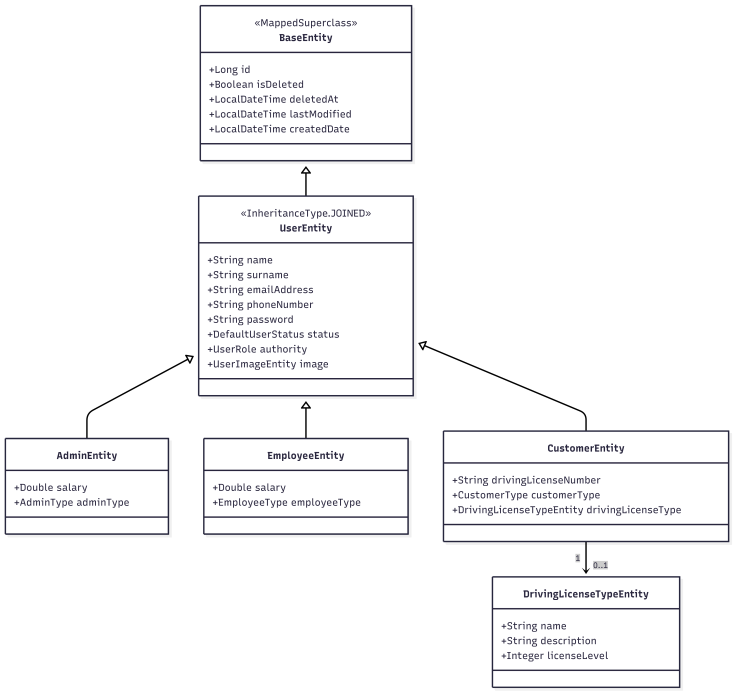
\includegraphics[width=0.82\textwidth]{cd_users.png}
        \caption{Class Diagram -- Gerarchia degli Utenti}
        \label{fig:cd-users}
    \end{figure}

% ── FIGURA 2 — GERARCHIA VEICOLI ─────────────────────────────────────────────
    \subsubsection*{Gerarchia dei Veicoli (Figura~\ref{fig:cd-vehicles})}

    \texttt{Vehicle} è una \textit{MappedSuperclass} astratta che raggruppa le
    caratteristiche generali di qualsiasi mezzo noleggiabile: anno di immatricolazione,
    numero di posti, capacità bagagli, prezzo giornaliero di noleggio e flag di
    disponibilità (\texttt{isAvailable}). Contiene inoltre riferimenti alle entità
    di classificazione (\texttt{ColorEntity}, \texttt{FuelTypeEntity},
    \texttt{ShiftTypeEntity}, \texttt{VehicleStatusEntity}) e al tipo di patente
    richiesta (\texttt{requiredLicenseType}), che viene confrontato con quello del
    cliente in fase di prenotazione.

    La classe concreta \textbf{\texttt{CarEntity}} estende \texttt{Vehicle}
    aggiungendo gli attributi specifici dell'automobile: targa (\texttt{licensePlate}),
    chilometraggio (\texttt{kilometer}), tipo di carrozzeria
    (\texttt{CarBodyTypeEntity}), segmento di mercato (\texttt{CarSegmentEntity})
    e modello (\texttt{CarModelEntity}). Quest'ultimo è a sua volta collegato a
    \texttt{BrandEntity}, che rappresenta il costruttore del veicolo (es.\
    Audi, BMW, Toyota) e ne conserva l'immagine su Cloudinary.

    \begin{figure}[H]
        \centering
        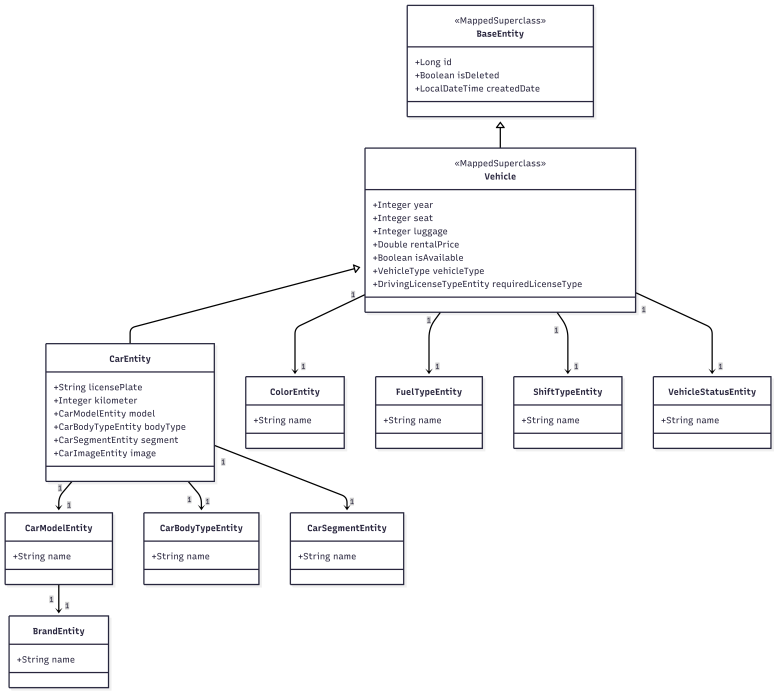
\includegraphics[width=0.90\textwidth]{cd_vehicles.png}
        \caption{Class Diagram -- Gerarchia dei Veicoli}
        \label{fig:cd-vehicles}
    \end{figure}

% ── FIGURA 3 — DOMINIO NOLEGGIO ───────────────────────────────────────────────
    \subsubsection*{Dominio del Noleggio e dei Pagamenti (Figura~\ref{fig:cd-rental})}

    \texttt{RentalEntity} è il fulcro del sistema e rappresenta un contratto di
    noleggio nella sua interezza. Essa aggrega un riferimento al cliente
    (\texttt{CustomerEntity}) e al veicolo noleggiato (\texttt{CarEntity}), le date
    di inizio, fine e restituzione effettiva, i chilometri di partenza e arrivo per
    il calcolo del percorso, lo stato corrente del noleggio (\texttt{RentalStatusEntity})
    e il flag \texttt{isActive} che indica se il noleggio è in corso.

    Il pagamento è modellato da \textbf{\texttt{PaymentDetailsEntity}}, associata
    in modo uno-a-uno a ogni noleggio: registra l'importo totale e il tipo di
    pagamento tramite \texttt{PaymentTypeEntity} (es.\ carta di credito, contanti,
    bonifico), anch'essa configurabile con stato attivo/inattivo. Opzionalmente,
    \texttt{RentalEntity} può essere collegata a una \textbf{\texttt{DiscountEntity}},
    che modella un codice sconto con percentuale configurabile e stato
    attivo/inattivo, permettendo al sistema di calcolare automaticamente l'importo
    scontato al momento della creazione del noleggio.

    \begin{figure}[H]
        \centering
        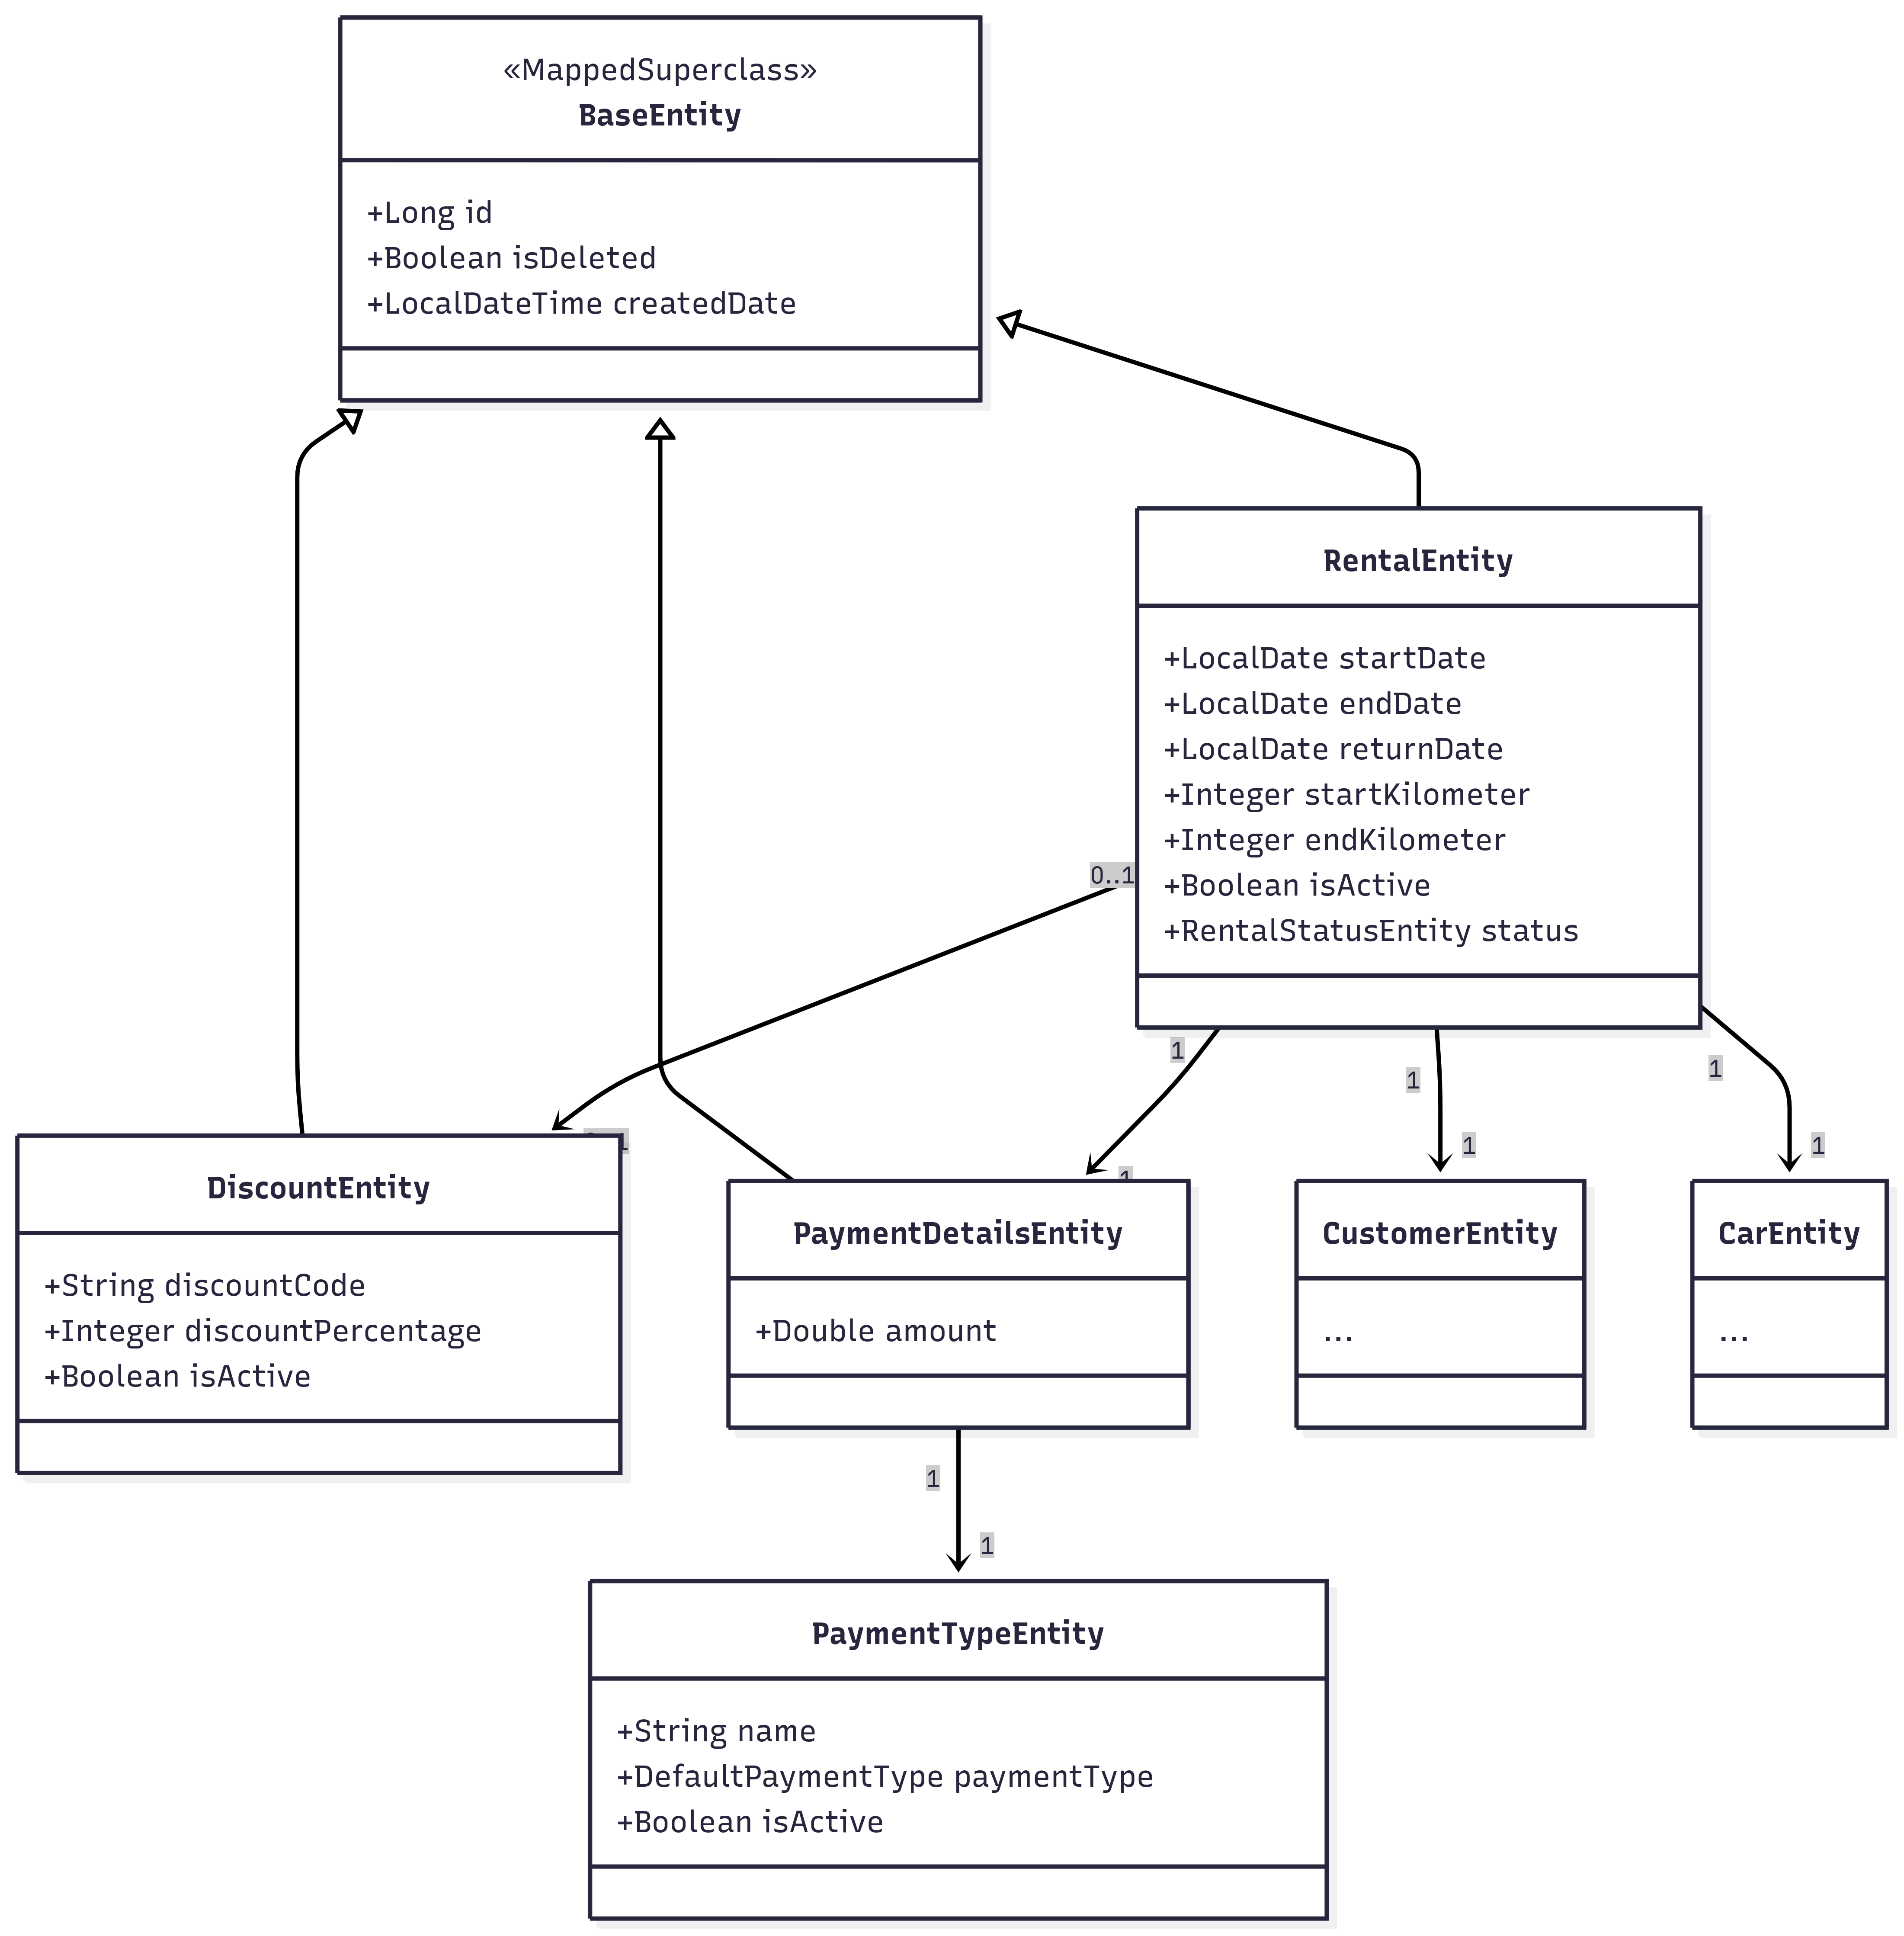
\includegraphics[width=0.72\textwidth]{cd_rental.png}
        \caption{Class Diagram -- Dominio del Noleggio e dei Pagamenti}
        \label{fig:cd-rental}
    \end{figure}
%
% =============================================================================
    \section{Frontend: Applicazione React}
    \label{sec:frontend}
% =============================================================================

    Il frontend di \textbf{ExtendRent} è una Single Page Application (SPA) sviluppata
    con \textbf{React 18} e \textbf{TypeScript}, che si interfaccia con il backend
    Spring Boot tramite API REST. L'applicazione è containerizzata con Docker e
    servita da nginx (descritto nella sezione~\ref{sec:docker}).

% ─────────────────────────────────────────────
    \subsection{Stack Tecnologico}
% ─────────────────────────────────────────────

    \begin{table}[H]
        \centering
        \small
        \begin{tabular}{lll}
            \toprule
            \textbf{Categoria} & \textbf{Tecnologia} & \textbf{Versione} \\
            \midrule
            Framework UI & React + TypeScript & 18.0.2 / 4.9.5 \\
            Routing & React Router DOM & 6.21.1 \\
            State management & Redux Toolkit & 2.0.1 \\
            HTTP client & Axios (con interceptors) & 1.6.5 \\
            Form handling & Formik + Yup & 2.4.5 / 1.3.3 \\
            UI libraries & Material UI, Mantine, Bootstrap & 5.15 / 7.4 / 5.3 \\
            Tabelle & material-react-table & 2.11.2 \\
            Date picker & @mantine/dates, @mui/x-date-pickers & 7.4 / 6.19 \\
            Animazioni & Framer Motion & 10.17 \\
            Token decoding & jwt-decode & 4.0.0 \\
            Build & Create React App + React Scripts & 5.0.1 \\
            \bottomrule
        \end{tabular}
        \caption{Stack tecnologico del frontend}
        \label{tab:frontend_stack}
    \end{table}

% ─────────────────────────────────────────────
    \subsection{Architettura e Struttura}
% ─────────────────────────────────────────────

    Il progetto segue un'architettura a strati:

    \begin{itemize}
        \item \textbf{\texttt{pages/}} --- 30+ pagine React suddivise per dominio
        funzionale. Includono pagine pubbliche (Homepage, Login, SignUp),
        pagine per utenti autenticati (Account, PastRentals) e pagine di
        amministrazione protette (\texttt{adminPanel/**}).
        \item \textbf{\texttt{components/}} --- Componenti riutilizzabili:
        \texttt{Navbar}, \texttt{Search}, \texttt{Payment},
        \texttt{CarCart}, \texttt{RentalDetail}, \texttt{OverlayLoader}
        (loading globale), \texttt{CreditCardForm}, \texttt{PasswordStrength}.
        \item \textbf{\texttt{store/}} --- Redux Toolkit store con 22 slice tematici
        (\texttt{carSlice}, \texttt{rentalSlice}, \texttt{signInSlice}, ecc.)
        e loading globale automatico via \texttt{addMatcher} su
        \texttt{pending}/\texttt{fulfilled}/\texttt{rejected}.
        \item \textbf{\texttt{services/}} --- Layer di comunicazione con il backend:
        20+ service class che incapsulano le chiamate Axios per ogni entità
        (Car, Rental, Customer, Brand, Color, ecc.).
        \item \textbf{\texttt{models/}} --- Modelli TypeScript tipizzati per tutte
        le request e response, garantendo type-safety end-to-end.
        \item \textbf{\texttt{utils/}} --- \texttt{axiosInterceptors.ts} (istanza
        Axios condivisa con \texttt{withCredentials: true}) e
        \texttt{useToken.ts} (hook per decodare i claim JWT).
    \end{itemize}

    \begin{lstlisting}[language=bash, caption={Struttura semplificata del frontend}]
rent-a-car-frontend-project/src/
|-- App.tsx               # Routing principale (React Router v6)
|-- index.tsx             # Entry point con Provider Redux
|-- pages/                # 30+ pagine per dominio
|   |-- Homepage/         # Pubblica: search + video background
|   |-- Login/ SignUp/    # Autenticazione
|   |-- AdminPanel/       # Dashboard admin (protetta)
|   |-- Cars/ Rental/     # CRUD auto e noleggi
|   |-- Customer/         # Gestione clienti
|   |-- PastRentals/      # Storico noleggi cliente
|   `-- [Brands, Colors, FuelType, Discount, Payment, ...]
|-- components/           # Componenti riutilizzabili
|-- store/                # Redux Toolkit (22 slice)
|-- services/             # Axios service classes (20+)
|-- models/               # TypeScript models (request/response)
|-- utils/                # axiosInterceptors, useToken
`-- data/config.json      # Base URL API
    \end{lstlisting}

% ─────────────────────────────────────────────
    \subsection{Autenticazione e Sicurezza Frontend}
% ─────────────────────────────────────────────

    Il frontend implementa un meccanismo di autenticazione allineato con le patch
    di sicurezza applicate al backend:

    \subsubsection*{HttpOnly Cookie}

    A seguito della patch \textbf{V02} (HttpOnly cookie), il frontend non memorizza
    più i token in \texttt{localStorage} (vettore XSS). La configurazione Axios
    centralizzata in \texttt{axiosInterceptors.ts} usa \texttt{withCredentials: true},
    che istruisce il browser a inviare automaticamente i cookie HttpOnly su ogni
    richiesta API:

    \begin{lstlisting}[language=Java, caption={axiosInterceptors.ts --- configurazione Axios}]
const axiosInstance = axios.create({
  baseURL: config.apiBaseUrl,
  withCredentials: true,  // invia cookie HttpOnly su ogni request
});
    \end{lstlisting}

    Il campo \texttt{token} restituito dal backend nel corpo della response di signin
    è ora vuoto (i token viaggiano esclusivamente via cookie); il frontend decodifica
    il JWT via \texttt{jwt-decode} per estrarre i claim (\texttt{id}, \texttt{role},
    \texttt{emailAddress}) necessari all'UI, senza mai esporre il token grezzo.

    \subsubsection*{RBAC Lato Frontend}

    Il controllo dei ruoli è implementato sia nella \texttt{Navbar} che nel componente
    \texttt{AdminRoutes}:

    \begin{itemize}
        \item \textbf{Navbar}: il link ``Admin Panel'' è visibile solo se
        \texttt{decodedToken.role} contiene \texttt{"ADMIN"}.
        \item \textbf{AdminRoutes}: componente di routing che blocca l'accesso alle
        route \texttt{/adminPanel/**} per utenti non ADMIN, reindirizzando alla
        homepage.
    \end{itemize}

    Il RBAC frontend è un livello di UX, non una misura di sicurezza primaria:
    il backend enforcement (via \texttt{SecurityConfig.hasRole("ADMIN")}) è la
    barriera reale contro accessi non autorizzati.

    \subsubsection*{Validazione Form}

    Tutti i form usano \textbf{Formik} con schemi \textbf{Yup} per la validazione
    client-side prima dell'invio:
    \begin{itemize}
        \item Password: lunghezza, complessità, visualizzata con \texttt{PasswordStrength}.
        \item Targa veicolo: regex formato.
        \item Email: schema Yup \texttt{.email()}.
        \item Date noleggio: vincoli temporali (data fine dopo data inizio).
        \item Dati carta di credito: validazione numero e CVV.
    \end{itemize}

% ─────────────────────────────────────────────
    \subsection{Pagine e Route Principali}
% ─────────────────────────────────────────────

    \begin{table}[H]
        \centering
        \small
        \begin{tabular}{|l|l|l|}
            \hline
            \textbf{Route} & \textbf{Accesso} & \textbf{Funzione} \\
            \hline
            \texttt{/} & Pubblico & Homepage con ricerca per date \\
            \texttt{/login} & Pubblico & Form di autenticazione \\
            \texttt{/signup} & Pubblico & Registrazione nuovi clienti \\
            \texttt{/selectedCar} & Pubblico & Dettaglio auto + checkout \\
            \texttt{/account} & Autenticato & Profilo personale \\
            \texttt{/allMyRentals/:id} & Autenticato & Storico noleggi \\
            \texttt{/adminPanel} & ADMIN & Dashboard \\
            \texttt{/adminPanel/cars} & ADMIN & CRUD auto \\
            \texttt{/adminPanel/rentals} & ADMIN & Gestione noleggi \\
            \texttt{/adminPanel/customers} & ADMIN & Gestione clienti \\
            \texttt{/adminPanel/employees} & ADMIN & Gestione dipendenti \\
            \texttt{/adminPanel/discountCodes} & ADMIN & Gestione codici sconto \\
            \texttt{/adminPanel/paymentDetails} & ADMIN & Dettagli pagamento \\
            \texttt{/adminPanel/[brands|colors|...]} & ADMIN & CRUD dati tecnici auto \\
            \hline
        \end{tabular}
        \caption{Principali route del frontend React}
        \label{tab:frontend_routes}
    \end{table}

% ─────────────────────────────────────────────
    \subsection{Flusso di Una Feature: Ricerca e Prenotazione Auto}
% ─────────────────────────────────────────────

    Il flusso principale dell'applicazione illustra come backend e frontend
    cooperano:

    \begin{enumerate}
        \item \textbf{Homepage} --- il componente \texttt{Search} raccoglie le date
        di inizio e fine noleggio tramite un date picker.
        \item \textbf{Redux Thunk} --- \texttt{getByAllFilteredCars()} chiama
        \texttt{GET /api/v1/cars/filter?startDate=\&endDate=} e salva i
        risultati nello store.
        \item \textbf{SelectedCar} --- mostra le auto disponibili; il componente
        \texttt{ShowRental} calcola il prezzo (con eventuale sconto via
        \texttt{POST /api/v1/rentals/show}) e il componente \texttt{Payment}
        raccoglie i dati della carta di credito.
        \item \textbf{Checkout} --- \texttt{POST /api/v1/rentals} crea il noleggio;
        la response aggiorna lo store e mostra il riepilogo.
    \end{enumerate}

% =============================================================================
    \section{Analisi delle Vulnerabilit\`a}
    \label{sec:vulnerabilities}
% =============================================================================

    L'analisi statica del codice sorgente è stata condotta in 4 sessioni di audit
    utilizzando l'\textbf{OWASP Top 10 2021} come framework di classificazione e il
    \textbf{CWE (Common Weakness Enumeration)} come riferimento tecnico per le debolezze
    individuate. Sono state identificate complessivamente \textbf{15 vulnerabilità}
    (14 specifiche, denominate V01--V14, più una falla architetturale, S1-1).
    Stato di partenza: 173 casi di test con \textbf{75 fallimenti}, poiché la catena
    di sicurezza globale era assente.

    \subsection{Riepilogo delle Vulnerabilità}

    \begin{table}[H]
        \centering
        \small
        \renewcommand{\arraystretch}{1.2}
        \begin{tabular}{|c|p{5.5cm}|c|c|p{1.8cm}|c|}
            \hline
            \textbf{ID} & \textbf{Titolo} & \textbf{Gravità} & \textbf{OWASP} & \textbf{CWE} & \textbf{Stato} \\
            \hline
            S1-1 & Global \texttt{permitAll()} --- nessun RBAC & Critica & A01 & 284, 862 & \checkmark \\
            V01  & Password nei query parameter & Critica & A07 & 598 & \checkmark \\
            V02  & Escalation ruolo via signup & Critica & A01 & 269 & \checkmark \\
            V03  & Domini attaccanti in whitelist CORS & Alta & A05 & 942 & \checkmark \\
            V04  & Credenziali hardcoded in \texttt{.properties} & Alta & A02 & 798 & \checkmark \\
            V05  & Refresh token loggato in chiaro & Alta & A09 & 532 & \checkmark \\
            V06  & Nessun rate limiting su auth endpoint & Alta & A07 & 307 & \checkmark \\
            V07  & Nessuna validazione tipo file upload & Alta & A03 & 434 & \checkmark \\
            V08  & Exception handler espone \texttt{e.getMessage()} & Media & A05 & 209 & \checkmark \\
            V09  & TTL identico per access e refresh token & Media & A07 & 613 & \checkmark \\
            V10  & Nessuna revoca server-side del refresh token & Media & A07 & 613 & \checkmark \\
            V11  & Password deboli per utenti di seed & Media & A07 & 521 & \checkmark \\
            V12  & Configurazione CORS duplicata & Bassa & A05 & 16 & \checkmark \\
            V13  & Swagger UI accessibile in produzione & Bassa & A05 & 16 & \checkmark \\
            V14  & Header \texttt{Content-Security-Policy} mancante & Media & A05 & 693 & \checkmark \\
            \hline
        \end{tabular}
        \caption{Riepilogo delle vulnerabilità identificate (15 totali, tutte risolte)}
        \label{tab:vulnerabilities}
    \end{table}

    \textbf{Distribuzione per gravità:} 3 critiche (S1-1, V01, V02),
    5 alte (V03--V07), 5 medie (V08--V11, V14), 2 basse (V12, V13).
    \textbf{Categorie OWASP coperte:} A01, A02, A03, A05, A07, A09.

    \subsection{Descrizione delle Vulnerabilità}

    \subsubsection{S1-1 --- Nessun Controllo di Accesso Globale (Critica)}
    \textbf{OWASP:} A01 \textbar{} \textbf{CWE:} CWE-284, CWE-862

    \texttt{SecurityConfig} impostava \texttt{anyRequest().permitAll()} come regola
    globale: ogni endpoint era accessibile senza autenticazione. Un attaccante anonimo
    poteva leggere o modificare qualsiasi dato.

    \subsubsection{V01 --- Password nei Query Parameter (Critica)}
    \textbf{OWASP:} A07 \textbar{} \textbf{CWE:} CWE-598

    \texttt{GET /isUserTrue?password=...} e \texttt{PUT /updatePassword?oldPassword=...}
    trasmettevano le password in chiaro nei log di accesso e nella cronologia del browser.

    \subsubsection{V02 --- Escalation di Ruolo via Signup Pubblico (Critica)}
    \textbf{OWASP:} A01 \textbar{} \textbf{CWE:} CWE-269

    \texttt{POST /api/v1/auth/signup} accettava \texttt{"authority": "ADMIN"} nel body,
    consentendo a un attaccante anonimo di creare un account amministratore.

    \subsubsection{V03 --- Domini Attaccanti nella Whitelist CORS (Alta)}
    \textbf{OWASP:} A05 \textbar{} \textbf{CWE:} CWE-942

    \texttt{CorsConfig.ALLOWED\_ORIGINS} conteneva \texttt{https://attacker.example.com}
    e \texttt{https://evil-attacker.com}, consentendo richieste cross-origin credenziate
    per leggere token JWT e dati personali.

    \subsubsection{V04 --- Credenziali Hardcoded (Alta)}
    \textbf{OWASP:} A02 \textbar{} \textbf{CWE:} CWE-798

    Sei credenziali di produzione committate in chiaro: password DB (\texttt{andrea72}),
    JWT secret HS256 noto (permetteva di forgiare token con qualsiasi ruolo),
    chiavi Cloudinary, password SMTP.

    \subsubsection{V05 --- Token Loggato in Chiaro (Alta)}
    \textbf{OWASP:} A09 \textbar{} \textbf{CWE:} CWE-532

    \texttt{RefreshTokenController} loggava \texttt{refreshTokenRequest.getToken()},
    esponendo il valore raw in log spesso inoltrati a sistemi esterni non cifrati.

    \subsubsection{V06 --- Nessun Rate Limiting (Alta)}
    \textbf{OWASP:} A07 \textbar{} \textbf{CWE:} CWE-307

    Nessuna limitazione su \texttt{/signin}, \texttt{/isUserTrue} e \texttt{/refresh-token}:
    brute-force illimitato e enumerazione email tramite l'oracolo booleano \texttt{isUserTrue}.

    \subsubsection{V07 --- Nessuna Validazione del Tipo di File (Alta)}
    \textbf{OWASP:} A03 \textbar{} \textbf{CWE:} CWE-434

    I service di upload accettavano qualsiasi file fidandosi del \texttt{Content-Type}
    fornito dal client, consentendo upload di HTML, JavaScript o eseguibili.

    \subsubsection{V08--V14}
    \textbf{V08} (CWE-209): exception handler esponeva nomi di classe e schema DB.
    \textbf{V09} (CWE-613): access e refresh token con lo stesso TTL di 24 ore.
    \textbf{V10} (CWE-613): refresh token stateless, nessuna revoca possibile dopo logout.
    \textbf{V11} (CWE-521): password seed \texttt{"pass"} (4 caratteri), bypassando \texttt{@Size(min=8)}.
    \textbf{V12} (CWE-16): CORS duplicata in \texttt{CorsConfig} e \texttt{WebConfig}.
    \textbf{V13} (CWE-16): path Swagger nella whitelist pubblica di \texttt{SecurityConfig}.
    \textbf{V14} (CWE-693): nessun header \texttt{Content-Security-Policy}, rischio clickjacking.

% =============================================================================
    \section{Mitigazione delle Vulnerabilit\`a}
    \label{sec:mitigations}
% =============================================================================

    Tutte e 15 le vulnerabilità sono state mitigate in 7 sessioni di lavoro
    (11--12 aprile 2026). Sono stati creati \textbf{7 nuovi file di produzione}
    e modificati oltre 10 file esistenti.

    \subsection{S1-1 --- Implementazione del Deny-by-Default RBAC}

    \begin{lstlisting}[language=Java, caption={SecurityConfig.java --- da permitAll a deny-by-default}]
// Prima (vulnerabile)
.anyRequest().permitAll()

// Dopo (sicuro)
.requestMatchers(DEFAULT_WHITE_LIST_URLS).permitAll()
.requestMatchers("/swagger-ui/**", "/v3/api-docs/**")
    .hasRole("ADMIN")                     // V13: Swagger solo admin
.requestMatchers(HttpMethod.POST, "/api/v1/auth/signup",
    "/api/v1/auth/signin",
    "/api/v1/auth/isUserTrue").permitAll()
.requestMatchers("/api/v1/verify/**").permitAll()
.requestMatchers(HttpMethod.POST, "/api/v1/refresh-token/**").permitAll()
.requestMatchers(HttpMethod.POST, "/api/v1/auth/logout").authenticated()
.requestMatchers("/api/v1/admins/**").hasRole("ADMIN")
.requestMatchers("/api/v1/users/**").hasRole("ADMIN")
.requestMatchers("/api/v1/employees/**").hasRole("ADMIN")
.requestMatchers("/api/v1/rentals/**").hasRole("ADMIN")
.requestMatchers("/api/v1/discounts/**").hasRole("ADMIN")
.requestMatchers("/api/v1/paymentDetails/**").hasRole("ADMIN")
.requestMatchers("/api/v1/paymentTypes/**").hasRole("ADMIN")
.requestMatchers("/api/v1/customers/**").hasRole("ADMIN")
.requestMatchers("/api/v1/images/**").hasRole("ADMIN")
.requestMatchers("/api/v1/brands/**").authenticated()
.requestMatchers("/api/v1/cars/**").authenticated()
// ... altri endpoint di catalogo -> authenticated()
.anyRequest().authenticated()
    \end{lstlisting}

    \subsection{V01 --- Rimozione delle Password dai Query Parameter}

    \begin{lstlisting}[language=Java, caption={AuthenticationController.java --- password in request body}]
// Prima (vulnerabile)
@GetMapping("/isUserTrue")
public Response<Boolean> isUserTrue(
    @RequestParam String email, @RequestParam String password)

// Dopo (sicuro)
@PostMapping("/isUserTrue")
public Response<Boolean> isUserTrue(
    @RequestBody IsUserTrueRequest request)
    \end{lstlisting}

    \subsection{V02 --- Prevenzione dell'Escalation di Ruolo}

    \begin{lstlisting}[language=Java, caption={SignUpReqeust.java --- validatore @AssertTrue}]
@AssertTrue(message = "Authority must be CUSTOMER")
public boolean isAuthorityCustomer() {
    return authority == null
        || authority.equals(UserAuthority.CUSTOMER);
}
    \end{lstlisting}

    \subsection{V04 --- Rimozione delle Credenziali Hardcoded}

    La mitigazione adotta un approccio a \textbf{due livelli}:

    \begin{itemize}
        \item \textbf{Sviluppo locale}: \texttt{application.properties} è aggiunto al
        \texttt{.gitignore} e non viene mai committato. Ogni sviluppatore mantiene
        un file locale (partendo da \texttt{application.properties.example}) con le
        proprie credenziali di sviluppo, mai condivise nel repository.
        \item \textbf{Deployment Docker}: \texttt{application-docker.properties} (committato,
        privo di credenziali) usa variabili d'ambiente e Docker Secrets per tutte le
        credenziali sensibili.
    \end{itemize}

    \begin{lstlisting}[language=bash, caption={application-docker.properties --- credenziali da Docker Secrets}]
# Sviluppo locale: application.properties (gitignored, credenziali dirette)
spring.datasource.password=<local-dev-password>   # mai committato

# Docker deployment: application-docker.properties (committato, senza credenziali)
spring.datasource.password=${DB_PASSWORD}
application.security.jwt.secret-key=${JWT_SECRET}
cloudinary.api-key=${CLOUDINARY_API_KEY}
cloudinary.api-secret=${CLOUDINARY_API_SECRET}
spring.mail.password=${MAIL_PASSWORD}
    \end{lstlisting}

    \subsection{V06 --- Rate Limiting con Bucket4j}

    Creato \texttt{RateLimitFilter extends OncePerRequestFilter} con algoritmo
    token-bucket (Bucket4j 8.10.1): 10 richieste/minuto per IP su tutti gli
    endpoint \texttt{/api/v1/auth/**} e \texttt{/api/v1/refresh-token}.
    HTTP 429 con header \texttt{Retry-After: 60} in caso di esaurimento.
    I bucket per IP sono gestiti da una cache Caffeine con TTL di 2 minuti
    e limite di 50.000 entry per prevenire memory exhaustion sotto attacchi
    con IP rotation. Il flag \texttt{app.rate-limit.enabled} consente la
    disabilitazione durante i test.

    \begin{lstlisting}[language=Java, caption={RateLimitFilter.java --- logica token-bucket con Caffeine}]
// Cache Caffeine: evicts stale IPs, bounded at 50,000 entries
private final Cache<String, Bucket> buckets = Caffeine.newBuilder()
        .expireAfterAccess(2, TimeUnit.MINUTES)
        .maximumSize(50_000)
        .build();

// Bucket per IP (Refill.greedy = ricarica continua, non batch)
Bucket bucket = buckets.get(ip, k ->
    Bucket.builder()
        .addLimit(Bandwidth.classic(10,
            Refill.greedy(10, Duration.ofMinutes(1))))
        .build());
if (!bucket.tryConsume(1)) {
    response.setStatus(429);
    response.setHeader("Retry-After", "60");
    return;
}
chain.doFilter(request, response);
    \end{lstlisting}

    \subsection{V10 --- Revoca Stateful del Refresh Token}

    \begin{lstlisting}[language=SQL, caption={Schema tabella refresh\_tokens}]
CREATE TABLE refresh_tokens (
  id         UUID PRIMARY KEY,
  token_hash VARCHAR(255) NOT NULL UNIQUE, -- SHA-256
  user_id    UUID NOT NULL REFERENCES users(id),
  issued_at  TIMESTAMP NOT NULL,
  expires_at TIMESTAMP NOT NULL,
  revoked    BOOLEAN DEFAULT FALSE
);
    \end{lstlisting}

    Il flusso implementa \textbf{token rotation} con rilevamento del furto:
    se un token già revocato viene riutilizzato, \texttt{revokeAllForUser()}
    invalida tutte le sessioni attive e forza una nuova autenticazione.

    \subsection{Ulteriori Mitigazioni}

    \begin{itemize}
        \item \textbf{V03}: rimossi domini attaccanti da \texttt{CorsConfig.ALLOWED\_ORIGINS}.
        \item \textbf{V05}: rimosso \texttt{token.getValue()} da \texttt{log.info()}.
        \item \textbf{V07}: whitelist Content-Type in \texttt{CarImageServiceImpl} e \texttt{UserImageServiceImpl}.
        \item \textbf{V08}: \texttt{e.getMessage()} sostituito con messaggio statico generico.
        \item \textbf{V09}: access token 1 ora (\texttt{expiration=3600000}), refresh token 7 giorni (\texttt{refresh-expiration=604800000}). \texttt{JwtService} usa \texttt{refreshExpiration} separato; i valori sono aggiornati in \texttt{application.properties} e \texttt{application-docker.properties}.
        \item \textbf{V11}: password seed da \texttt{"pass"} a \texttt{"Seed@1234"}.
        \item \textbf{V12}: rimosso \texttt{addCorsMappings()} da \texttt{WebConfig.java}.
        \item \textbf{V13}: path Swagger spostati sotto \texttt{.hasRole("ADMIN")} (restrizione più forte di \texttt{.authenticated()}: solo admin può accedere alla documentazione API).
        \item \textbf{V14}: aggiunto CSP: \texttt{default-src 'self'; frame-ancestors 'none'}.
    \end{itemize}

    \subsection{Mitigazioni Architetturali Aggiuntive}

    Oltre alle patch per le vulnerabilità identificate, sono state introdotte ulteriori
    misure di sicurezza non originalmente previste:

    \begin{itemize}
        \item \textbf{HttpOnly Cookie per i token}: l'endpoint \texttt{POST /api/v1/auth/signin}
        non restituisce più access e refresh token nel corpo della risposta, bensì li imposta
        come cookie \texttt{HttpOnly; Secure; SameSite=Strict}. Questo elimina l'accesso
        JavaScript ai token (protezione XSS) e riduce la superficie per token theft.
        Il cookie di refresh ha path ristretto a \texttt{/api/v1/refresh-token}.

        \item \textbf{Endpoint di Logout}: aggiunto \texttt{POST /api/v1/auth/logout}
        (richiede autenticazione) che revoca tutti i refresh token dell'utente e scade
        immediatamente i cookie impostando \texttt{maxAge=0}.

        \item \textbf{Profilo \texttt{application-docker.properties}}: aggiunto profilo Spring
        dedicato al deployment Docker (\texttt{SPRING\_PROFILES\_ACTIVE=docker}) che legge le
        credenziali da Docker Secrets via \texttt{spring.config.import=optional:configtree:/run/secrets/}.
        Questo sostituisce la necessità di env vars esplicite e riduce la superficie di
        esposizione tramite \texttt{docker inspect}.
    \end{itemize}

% ==================================================================================
% SEZIONE: TEST DI SICUREZZA
% ==================================================================================

    \section{Test di Sicurezza}
    \label{sec:security_testing}

% ==================================================================================
    \subsection{Introduzione}
    \label{subsec:security_intro}

    I test di sicurezza rappresentano una componente critica della pipeline di verifica
    del progetto RentACar. La suite di sicurezza comprende \textbf{231 casi di test} nel package
    \texttt{com.extendrent.security}, organizzati in 8 macrogruppi tematici,
    ciascuno focalizzato su una specifica classe di vulnerabilità conforme al
    framework OWASP Top 10 2021.

    \textbf{Stato finale (2026-04-18):}
    \begin{itemize}
        \item Totale test di sicurezza: 231
        \item Pass: 231 (100\%)
        \item Fail: 0
        \item Skipped: 0
    \end{itemize}

    Il 100\% dei test è verde. Tutte le 15 vulnerabilità identificate durante l'analisi
    statica sono state patchate con corrispondenti test di regressione.

    Lo scopo della suite è verificare che l'applicazione implementi correttamente:
    \begin{enumerate}
        \item Controlli di accesso (RBAC, autorizzazione per endpoint/metodo HTTP)
        \item Protezione dei dati sensibili (credenziali, token, PII)
        \item Gestione degli errori senza esposizione di informazioni critiche
        \item Resistenza agli attacchi comuni (brute-force, CORS, privilege escalation)
        \item Conformità ai vincoli di sicurezza (TTL token, logging sicuro, validazione input)
    \end{enumerate}

% ==================================================================================
    \subsection{Architettura della Suite di Test}
    \label{subsec:security_architecture}

    \subsubsection{Struttura di progetto}

    I test di sicurezza sono organizzati in \texttt{src/test/java/com/extendrent/security/}
    con 30 classi di test:

    \begin{table}[H]
        \centering
        \small
        \begin{tabular}{|p{8cm}|p{10cm}|}
            \hline
            \textbf{Classe di test} & \textbf{Ambito} \\
            \hline
            \texttt{AccountLockoutSecurityTest} & Blocco account dopo N tentativi falliti \\
            \texttt{AdminControllerSecurityTest} & ACL su /api/v1/admins/** \\
            \texttt{AuthenticationControllerSecurityTest} & Validazione input auth, error handling, file upload \\
            \texttt{CorsSecurityTest} & CORS misconfiguration, CSP header, wildcard \\
            \texttt{CorsAttackerDomainSecurityTest} & Domini ostili in CORS whitelist (V03) \\
            \texttt{CorsConfigDuplicationSecurityTest} & CORS duplicata (V12) \\
            \texttt{EmployeeControllerSecurityTest} & ACL su /api/v1/employees/** \\
            \texttt{GenericExceptionHandlerSecurityTest} & Exception disclosure (V08) \\
            \texttt{HardcodedCredentialsSecurityTest} & Credenziali hardcoded, gitignore (V04) \\
            \texttt{HttpOnlyCookieSecurityTest} & Cookie HttpOnly per access/refresh token \\
            \texttt{InputValidationSecurityTest} & Validazione query param, payload JSON, upload \\
            \texttt{JwtAuthFilterTest} & Token parsing, firma, scadenza \\
            \texttt{JwtClaimsPIISecurityTest} & PII nei claim JWT (no email/password in payload) \\
            \texttt{JwtServiceTest} & Generazione token, claim, validazione crittografica \\
            \texttt{JwtTtlSecurityTest} & TTL access token vs refresh token (V09) \\
            \texttt{LogoutSecurityTest} & Logout revoca token e scade cookie \\
            \texttt{PasswordComplexitySecurityTest} & Complessità password signup \\
            \texttt{PaymentValidationSecurityTest} & Validazione dati pagamento \\
            \texttt{RateLimitXForwardedForSecurityTest} & X-Forwarded-For spoofing e trusted proxy \\
            \texttt{RateLimitingBehaviorTest} & Comportamento rate limit per-IP (V06) \\
            \texttt{RateLimitingSecurityTest} & Struttura rate limit via reflection (V06) \\
            \texttt{RefreshTokenLoggingSecurityTest} & Token in log (V05) \\
            \texttt{RefreshTokenRevocationSecurityTest} & Revoca, rotazione, theft detection (V10) \\
            \texttt{RentalControllerSecurityTest} & RBAC completo ciclo vita noleggio \\
            \texttt{RoleEscalationSecurityTest} & Role escalation signup (V02) \\
            \texttt{SecurityFilterChainTest} & Catena globale RBAC (S1-1) \\
            \texttt{SwaggerAdminOnlySecurityTest} & Swagger accessibile solo ad ADMIN (V13) \\
            \texttt{SwaggerProdAccessSecurityTest} & Swagger richiede autenticazione (V13) \\
            \texttt{UserControllerSecurityTest} & ACL su /api/v1/users/**, IDOR \\
            \texttt{ValidationErrorExposureSecurityTest} & Messaggi di errore non espongono info interne \\
            \hline
        \end{tabular}
        \caption{Classi di test di sicurezza (30 classi nel package \texttt{security/})}
        \label{tab:security_test_classes}
    \end{table}

    \subsubsection{Strategia di test per livelli (Defense in Depth)}

    La suite implementa quattro livelli di testing per coprire la superficie di attacco:

    \begin{description}
        \item[Livello 1 — Unit Security Test:] Validazione token scaduto/malformato/non firmato,
        parser JWT, utility autenticazione, mapper errori. \textit{Esempio:} \texttt{JwtAuthFilterTest}
        verifica che token scaduto restituisca 401.

        \item[Livello 2 — Web-layer Security Test:] ACL per endpoint/metodo HTTP, verifiche RBAC,
        gestione errori (400, 401, 403, 415, 429). Utilizza \texttt{@WebMvcTest} per isolamento.
        \textit{Esempio:} \texttt{AdminControllerSecurityTest} verifica che anonimo riceva 401
        e customer riceva 403 su read admin.

        \item[Livello 3 — Integration Security Test:] Catena completa con \texttt{@SpringBootTest},
        ownership check, token refresh, flussi reali con DB test. \textit{Esempio:} verifica che
        customer A non veda dati di customer B.

        \item[Livello 4 — Negative Security Test:] Payload malevoli, token alterati, path tampering,
        abuse di query parameter, rate limiting, brute-force. \textit{Esempio:} file HTML come immagine,
        credential in query string.
    \end{description}

% ==================================================================================
    \subsection{Macrogruppi di Test e Copertura Vulnerabilità}
    \label{subsec:security_test_groups}

    I 231 test di sicurezza sono organizzati in 8 macrogruppi tematici:

    \subsubsection{Macrogruppo 1: Broken Access Control (RBAC e Autorizzazione)}
    \label{subsubsec:group1_access_control}

    \textbf{Scope:} 87 test | \textbf{OWASP:} A01 | \textbf{CWE:} CWE-862, CWE-284, CWE-285

    Cosa viene testato:
    \begin{itemize}
        \item Endpoint admin bloccati su accesso anonimo (deve tornare 401)
        \item Endpoint admin bloccati su ruolo CUSTOMER (deve tornare 403)
        \item Endpoint write (POST, PUT, DELETE) richiedono solo ADMIN
        \item Role escalation tramite signup pubblico (V02)
        \item Hard delete e operazioni privilegiate
        \item IDOR (Insecure Direct Object Reference) implicito su update password
    \end{itemize}

    Classi di test coinvolte:
    \begin{itemize}
        \item \texttt{AdminControllerSecurityTest} (14 test)
        \item \texttt{RoleEscalationSecurityTest} (3 test)
        \item \texttt{EmployeeControllerSecurityTest} (12 test)
        \item \texttt{RentalControllerSecurityTest} (18 test)
        \item \texttt{UserControllerSecurityTest} (15 test)
        \item \texttt{SecurityFilterChainTest} (25 test)
    \end{itemize}

    Vulnerabilità coperte:
    \begin{itemize}
        \item \textbf{V02} — Role escalation su signup (FIXATA)
        \item \textbf{S1-1} — Policy globale RBAC (FIXATA in sessione 1)
        \item \textbf{IDOR implicito} — UpdatePassword senza ownership check
    \end{itemize}

    \textbf{Stato:} \checkmark{} \textbf{87/87 test PASS (100\%)} | 0 FAIL

    Esempi di test critico:
    \begin{lstlisting}[language=Java,caption=RoleEscalationSecurityTest — signup con ADMIN]
@Test
void signup_withAdminAuthority_mustBeRejected() throws Exception {
    String body = """
        {
          "firstName": "hacker",
          "email": "hacker@evil.com",
          "password": "password123",
          "authority": "ADMIN"
        }
        """;

    mockMvc.perform(post("/api/v1/auth/signup")
            .contentType(MediaType.APPLICATION_JSON)
            .content(body))
        .andExpect(status().isBadRequest())
        .andExpect(jsonPath("$.message").value(containsString("CUSTOMER")));
}
    \end{lstlisting}

    ---

    \subsubsection{Macrogruppo 2: Security Misconfiguration (CORS, Header, Config)}
    \label{subsubsec:group2_misconfiguration}

    \textbf{Scope:} 18 test | \textbf{OWASP:} A05 | \textbf{CWE:} CWE-942, CWE-16

    Cosa viene testato:
    \begin{itemize}
        \item CORS wildcard (\texttt{*}) non consentito
        \item Domini attaccanti non in whitelist (\texttt{evil-attacker.com}, \texttt{attacker.example.com})
        \item CORS non duplicata (un solo bean \texttt{WebMvcConfigurer})
        \item Swagger UI protetto in produzione
        \item Preflight request da origin non autorizzate non restituisce header CORS
    \end{itemize}

    Classi di test:
    \begin{itemize}
        \item \texttt{CorsSecurityTest} (10 test)
        \item \texttt{CorsAttackerDomainSecurityTest} (4 test)
        \item \texttt{CorsConfigDuplicationSecurityTest} (2 test)
        \item \texttt{SwaggerProdAccessSecurityTest} (2 test)
    \end{itemize}

    Vulnerabilità coperte:
    \begin{itemize}
        \item \textbf{V03} — Domini attaccanti in whitelist CORS (FIXATA)
        \item \textbf{V12} — Configurazione CORS duplicata (FIXATA)
        \item \textbf{V13} — Swagger UI pubblico (FIXATA)
    \end{itemize}

    \textbf{Stato:} \checkmark{} \textbf{18/18 test PASS (100\%)} | 0 FAIL

    Impatto di V03: Un attaccante servendo codice da \texttt{https://evil-attacker.com}
    poteva leggere il payload completo delle API (token JWT, dati personali) tramite CSRF
    cross-origin.

    ---

    \subsubsection{Macrogruppo 3: Cryptographic Failures e Secrets Management}
    \label{subsubsec:group3_cryptographic}

    \textbf{Scope:} 5 test | \textbf{OWASP:} A02 | \textbf{CWE:} CWE-798

    Cosa viene testato:
    \begin{itemize}
        \item Nessuna password DB hardcoded (controllo di \texttt{application.properties})
        \item Nessun JWT secret hardcoded
        \item Nessun API secret Cloudinary hardcoded
        \item Nessun SMTP password hardcoded
        \item Tutte le credenziali sostituite con placeholder \texttt{\$\{ENV\_VAR\}}
    \end{itemize}

    Classi di test:
    \begin{itemize}
        \item \texttt{HardcodedCredentialsSecurityTest} (5 test)
    \end{itemize}

    Vulnerabilità coperte:
    \begin{itemize}
        \item \textbf{V04} — Credenziali hardcoded (FIXATA — spostamento a env vars)
    \end{itemize}

    \textbf{Stato:} \checkmark{} \textbf{5/5 test PASS (100\%)} | 0 FAIL

    Patch applicata: 6 credenziali ruotate (DB, JWT, Cloudinary x2, SMTP, plus 1 aggiuntivo)
    e sostituite con placeholder \texttt{spring.datasource.password=\$\{DB\_PASSWORD\}}.

    ---

    \subsubsection{Macrogruppo 4: Identification and Authentication Failures}
    \label{subsubsec:group4_authentication}

    \textbf{Scope:} 17 test | \textbf{OWASP:} A07 | \textbf{CWE:} CWE-307, CWE-613, CWE-521

    Cosa viene testato:
    \begin{itemize}
        \item \textbf{V06} — Rate limiting su \texttt{/api/v1/auth/**} (FIXATA — Bucket4j)
        \item Access token TTL $\leq$ 1 ora
        \item Refresh token TTL $\gg$ access token (7 giorni vs 1 ora)
        \item Password seed non deboli ($\geq$ 8 caratteri, non \texttt{"pass"})
        \item Refresh token revocato dopo logout/cambio password (V10 — FIXATA)
    \end{itemize}

    Classi di test:
    \begin{itemize}
        \item \texttt{RateLimitingBehaviorTest} (4 test — PASS)
        \item \texttt{RateLimitingSecurityTest} (4 test — PASS)
        \item \texttt{JwtTtlSecurityTest} (3 test — PASS)
        \item \texttt{RefreshTokenRevocationSecurityTest} (6 test — PASS)
    \end{itemize}

    Vulnerabilità coperte:
    \begin{itemize}
        \item \textbf{V06} — Rate limiting (FIXATA con Bucket4j)
        \item \textbf{V09} — TTL identico access/refresh (FIXATA)
        \item \textbf{V10} — Revoca token (FIXATA con RefreshTokenEntity)
        \item \textbf{V11} — Password seed deboli (FIXATA)
    \end{itemize}

    \textbf{Stato:} \checkmark{} \textbf{17/17 test PASS (100\%)} | 0 FAIL

    Impatto di V06: Un attaccante poteva inviare 10.000 richieste/sec a \texttt{/api/v1/auth/signin}
    per brute-force credenziali. \texttt{isUserTrue} è un oracolo booleano per enumerazione email.

    ---

    \subsubsection{Macrogruppo 5: Security Logging and Monitoring Failures}
    \label{subsubsec:group5_logging}

    \textbf{Scope:} 5 test | \textbf{OWASP:} A09 | \textbf{CWE:} CWE-532, CWE-209

    Cosa viene testato:
    \begin{itemize}
        \item Refresh token non loggato in chiaro nei log dell'app
        \item Exception message generico in risposta 500 (non espone CWE, nomi classi)
        \item Stack trace completo conservato in log server-side (per debug interno)
    \end{itemize}

    Classi di test:
    \begin{itemize}
        \item \texttt{RefreshTokenLoggingSecurityTest} (2 test)
        \item \texttt{GenericExceptionHandlerSecurityTest} (3 test)
    \end{itemize}

    Vulnerabilità coperte:
    \begin{itemize}
        \item \textbf{V05} — Token loggato in chiaro (FIXATA)
        \item \textbf{V08} — 500 espone e.getMessage() (FIXATA)
    \end{itemize}

    \textbf{Stato:} \checkmark{} \textbf{5/5 test PASS (100\%)} | 0 FAIL

    Patch: rimozione di \texttt{log.info(REFRESH\_TOKEN\_REQUEST\_RECEIVED, token.getValue())}
    da \texttt{RefreshTokenController}.

    ---

    \subsubsection{Macrogruppo 6: Injection and Input Validation}
    \label{subsubsec:group6_injection}

    \textbf{Scope:} 34 test | \textbf{OWASP:} A03, A04 | \textbf{CWE:} CWE-20, CWE-434

    Cosa viene testato:
    \begin{itemize}
        \item Payload JSON malformato → 400 (non 500)
        \item Content-Type mancante su POST → 415 (non 500)
        \item Query parameter non numerico → 400 (non 500)
        \item Parameter obbligatorio mancante → 400 (non 500)
        \item File upload non immagine → 415/400, non 200 (V07 — protezione incidentale)
        \item Magic bytes immagini non validati (V07 — protezione incidentale, Tika raccomandato)
    \end{itemize}

    Classi di test:
    \begin{itemize}
        \item \texttt{AuthenticationControllerSecurityTest} (20 test)
        \item \texttt{InputValidationSecurityTest} (13 test — include validazione upload)
        \item \texttt{PasswordComplexitySecurityTest} (1 test)
    \end{itemize}

    Vulnerabilità coperte:
    \begin{itemize}
        \item \textbf{V07} — Validazione magic bytes immagini (PROTEZIONE INCIDENTALE)
    \end{itemize}

    \textbf{Stato:} \checkmark{} \textbf{34/34 test PASS (100\%)} | 0 FAIL

    Nota su V07: I test passano perché \texttt{ImageUtils.resizeImage()} lancia eccezione
    su file non-immagine, ma un \textbf{file polyglot} (JPEG valido + payload EXIF) supererebbe
    il controllo. Raccomandazione: usare Apache Tika per validazione magic bytes esplicita.

    ---

    \subsubsection{Macrogruppo 7: JWT and Token Management}
    \label{subsubsec:group7_jwt}

    \textbf{Scope:} 30 test | \textbf{OWASP:} A07 | \textbf{CWE:} CWE-613, CWE-347

    Cosa viene testato:
    \begin{itemize}
        \item Token scaduto rifiutato (401, non 200)
        \item Token malformato rifiutato (401)
        \item Token non firmato rifiutato (401)
        \item Signature invalida rifiutata (401)
        \item Claim mancante rifiutato (401)
        \item JWT secret sufficientemente lungo ($\geq$ 64 hex char = 32 byte)
        \item Claim fabricati non accettati (es. ruolo ADMIN da client)
        \item TTL access token $\leq$ 1 ora
        \item TTL refresh token $\gg$ access token
    \end{itemize}

    Classi di test:
    \begin{itemize}
        \item \texttt{JwtAuthFilterTest} (8 test)
        \item \texttt{JwtServiceTest} (19 test)
        \item \texttt{JwtTtlSecurityTest} (3 test)
    \end{itemize}

    Vulnerabilità coperte:
    \begin{itemize}
        \item \textbf{V09} — TTL identico access/refresh (FIXATA — 1h vs 7d)
    \end{itemize}

    \textbf{Stato:} \checkmark{} \textbf{30/30 test PASS (100\%)} | 0 FAIL

    Patch: separazione TTL in \texttt{JwtService.java} con proprietà \texttt{application.security.jwt.refresh-expiration}.

    ---

    \subsubsection{Macrogruppo 8: Application-specific (Payment, Image, Customer Data)}
    \label{subsubsec:group8_application_specific}

    \textbf{Scope:} 4 test implementati / 60+ target | \textbf{Coverage:} ~7\% (GAP ALTO)

    Cosa dovrebbe essere testato (target futuro):
    \begin{itemize}
        \item \texttt{PaymentDetailController} — accesso anonimo → 401; CUSTOMER → 403; ADMIN → 200
        \item \texttt{CustomerController} — CUSTOMER vede solo i propri dati (ownership); non cancella
        \item \texttt{ImageController} — upload validazione, rate limiting, spazio disco
        \item Controller veicoli (Brand, CarModel, Fuel) — read pubblico, write ADMIN-only
        \item \texttt{DiscountController} — creazione codici solo ADMIN
    \end{itemize}

    Classi di test:
    \begin{itemize}
        \item \texttt{PaymentValidationSecurityTest} (4 test)
        \item \textbf{MANCANTI:} CustomerControllerSecurityTest
        \item \textbf{MANCANTI:} ImageControllerSecurityTest
        \item \textbf{MANCANTI:} VehicleControllerSecurityTest
    \end{itemize}

    \textbf{Stato:} $\times$ \textbf{4/4 test PASS (100\%)} | 0 FAIL | \textbf{GAP: 56+ test non scritti}

    Priorità di remediation:
    \begin{enumerate}
        \item PaymentDetailController (dati finanziari — criticità alta)
        \item CustomerController (PII, IDOR — criticità alta)
        \item ImageController (upload DOS — criticità media)
        \item Vehicle controllers (catalogo pubblico vs admin — criticità media)
    \end{enumerate}

% ==================================================================================
    \subsection{Mappatura OWASP/CWE}
    \label{subsec:owasp_cwe_mapping}

    \subsubsection{Copertura OWASP Top 10 2021}

    La tabella seguente mostra come i test di sicurezza ricoprono le categorie OWASP
    Top 10 2021:

    \begin{table}[H]
        \centering
        \small
        \begin{tabular}{|c|l|c|c|c|}
            \hline
            \textbf{OWASP} & \textbf{Descrizione} & \textbf{Test} & \textbf{Vulnerabilità} & \textbf{Stato} \\
            \hline
            A01 & Broken Access Control & 87 & S1-1, V02, IDOR & \checkmark{} Coperto \\
            A02 & Cryptographic Failures & 5 & V04 & \checkmark{} Coperto \\
            A03 & Injection & 37 & V07 & \textbf{!} Incidentale \\
            A04 & Insecure Design & — & — & $\times$ Non coperto \\
            A05 & Security Misconfiguration & 18 & V03, V12, V13 & \checkmark{} Coperto \\
            A06 & Vulnerable/Outdated Components & — & — & — (scanning) \\
            A07 & Authentication Failures & 47 & V06, V09, V10, V11 & \checkmark{} Coperto \\
            A08 & Data Integrity Failures & — & — & $\times$ Non coperto \\
            A09 & Logging Failures & 4 & V05, V08 & \checkmark{} Coperto \\
            A10 & SSRF & — & — & $\times$ Non rilevante \\
            \hline
        \end{tabular}
        \caption{Copertura OWASP Top 10 2021}
        \label{tab:owasp_coverage}
    \end{table}

    Riepilogo:
    \begin{itemize}
        \item \textbf{Coperto completamente:} A01, A02, A05, A09
        \item \textbf{Parzialmente coperto:} A03 (protezione incidentale), A07 (V06/V10 aperti)
        \item \textbf{Non coperto:} A04 (insecure design — out of scope test), A06 (dependencies), A08 (data integrity), A10 (SSRF — no outbound client)
    \end{itemize}

    \subsubsection{Mappatura CWE (Common Weakness Enumeration)}

    \begin{table}[H]
        \centering
        \small
        \begin{tabular}{|c|l|l|c|}
            \hline
            \textbf{CWE ID} & \textbf{Titolo} & \textbf{Test} & \textbf{Vulnerabilità} \\
            \hline
            CWE-16 & Configuration & CorsConfigDuplicate, SwaggerProd & V12, V13 \\
            CWE-20 & Improper Input Validation & InputValidation & V07 \\
            CWE-209 & Information Exposure (Error) & GenericExceptionHandler & V08 \\
            CWE-269 & Improper Privilege Management & RoleEscalation & V02 \\
            CWE-284 & Improper Access Control & SecurityFilterChain & S1-1 \\
            CWE-285 & Improper Authorization & Rental, Employee & S1-1 \\
            CWE-307 & Excessive Auth Attempts & RateLimiting & V06 \\
            CWE-434 & Unrestricted File Upload & InputValidation & V07 \\
            CWE-532 & Sensitive Info in Log & RefreshTokenLogging & V05 \\
            CWE-613 & Insufficient Session Expiration & JwtTtl, RefreshToken & V09, V10 \\
            CWE-942 & Permissive Cross-domain Policy & CorsAttackerDomain & V03 \\
            \hline
        \end{tabular}
        \caption{Mappatura CWE — Test e Vulnerabilità}
        \label{tab:cwe_mapping}
    \end{table}

% ==================================================================================
    \subsection{Statistiche e Metriche Attuali}
    \label{subsec:metrics}

    \subsubsection{Riepilogo numerico}

    \begin{table}[H]
        \centering
        \begin{tabular}{|l|c|}
            \hline
            \textbf{Metrica} & \textbf{Valore} \\
            \hline
            Totale test di sicurezza & 231 \\
            Pass & 231 (100\%) \\
            Fail & 0 \\
            Skipped & 0 \\
            \hline
            Classi di test security & 30 \\
            \hline
            Vulnerabilità identificate & 15 \\
            Vulnerabilità fixate & 15 \\
            Vulnerabilità aperte & 0 \\
            Test di regressione aggiunti & 30 \\
            \hline
            Coverage OWASP A\# & 6 categorie completamente \\
            Coverage CWE & 16 CWE mappate \\
            \hline
        \end{tabular}
        \caption{Statistiche Suite di Sicurezza (2026-04-18)}
        \label{tab:security_stats}
    \end{table}

    \subsubsection{Distribuzione test per macrogruppo}

    \begin{table}[H]
        \centering
        \small
        \begin{tabular}{|l|c|c|l|}
            \hline
            \textbf{Macrogruppo} & \textbf{OWASP} & \textbf{Test} & \textbf{Classi principali} \\
            \hline
            Broken Access Control & A01 & 87 & SecurityFilterChain(25), Rental(18), User(15)... \\
            Security Misconfiguration & A05 & 18 & CorsSecurityTest(10), Attacker(4)... \\
            Cryptographic Failures & A02 & 5 & HardcodedCredentials(5) \\
            Authentication Failures & A07 & 23 & RateLimiting(8+6), JwtTtl(3), Revocation(6) \\
            Logging Failures & A09 & 5 & RefreshTokenLogging(2), ExceptionHandler(3) \\
            Injection \& Input Validation & A03 & 34 & AuthController(20), InputValidation(13), Complexity(1) \\
            JWT \& Token Management & A07 & 35 & JwtService(19), JwtAuthFilter(8), JwtTtl(3)... \\
            Application-specific & Vario & 24 & HttpOnlyCookie(4), Logout(4), JwtClaims(5)... \\
            \hline
        \end{tabular}
        \caption{Distribuzione test per macrogruppo (alcune classi coprono più macrogruppi; totale suite: 231 test)}
        \label{tab:test_distribution}
    \end{table}

% ==================================================================================
    \subsection{Vulnerabilità Patchate e Loro Test di Regressione}
    \label{subsec:patched_vulnerabilities}

    In questa sezione sono documentate le 11 vulnerabilità patchate, con dettagli di patch
    e test di regressione. La sessione 1 ha fixato problemi RBAC e CORS; la sessione 2
    ha fixato vulnerabilità specifiche identificate nell'analisi statica.

    \subsubsection{V02 — Escalation di Ruolo tramite Signup Pubblico}

    \textbf{Gravità:} Critica | \textbf{OWASP:} A01 | \textbf{CWE:} CWE-269

    \textbf{Descrizione:} L'endpoint pubblico \texttt{POST /api/v1/auth/signup} accettava
    un campo \texttt{authority} dove il chiamante anonimo poteva specificare il ruolo
    (ADMIN, EMPLOYEE, CUSTOMER). Un attaccante inviava \texttt{"authority": "ADMIN"}
    e otteneva un account amministratore.

    \textbf{File vulnerabile:}
    \begin{itemize}
        \item \texttt{SignUpReqeust.java}
        \item \texttt{CustomAuthenticationServiceImpl.java}
    \end{itemize}

    \textbf{Patch applicata:}
    \begin{enumerate}
        \item Aggiunto validatore \texttt{@AssertTrue} in \texttt{SignUpReqeust.isAuthorityCustomer()}
        \item Se \texttt{authority != CUSTOMER}, lancia \texttt{MethodArgumentNotValidException} (HTTP 400)
        \item Semplificato \texttt{CustomAuthenticationServiceImpl.signUp()} per forzare CUSTOMER
    \end{enumerate}

    \textbf{Test di regressione:}
    \begin{itemize}
        \item \texttt{RoleEscalationSecurityTest.signup\_withAdminAuthority\_mustBeRejected()} → \checkmark{} PASS
        \item \texttt{RoleEscalationSecurityTest.signup\_withEmployeeAuthority\_mustBeRejected()} → \checkmark{} PASS
    \end{itemize}

    \textbf{Impact:} Critica (100\% app compromise) → Post-patch: Mitigata completamente

    ---

    \subsubsection{V03 — Domini Controllati dall'Attaccante in Whitelist CORS}

    \textbf{Gravità:} Alta | \textbf{OWASP:} A05 | \textbf{CWE:} CWE-942

    \textbf{Descrizione:} La configurazione CORS includeva esplicitamente:
    \begin{itemize}
        \item \texttt{https://attacker.example.com}
        \item \texttt{https://evil-attacker.com}
    \end{itemize}

    Uno script servito da questi domini poteva leggere il payload completo delle API
    (token JWT, dati personali) tramite richieste cross-origin credenziate.

    \textbf{Patch applicata:}
    \begin{enumerate}
        \item Rimossi i due domini dal campo \texttt{ALLOWED\_ORIGINS} in \texttt{CorsConfig.java}
        \item Rimosso metodo \texttt{addCorsMappings()} da \texttt{WebConfig.java} (duplicazione)
    \end{enumerate}

    \textbf{Test di regressione:}
    \begin{itemize}
        \item \texttt{CorsAttackerDomainSecurityTest.preflight\_fromEvilAttackerCom\_mustBeRejected()} → \checkmark{} PASS
        \item \texttt{CorsAttackerDomainSecurityTest.simpleRequest\_fromEvilAttackerCom\_mustNotReflectAcao()} → \checkmark{} PASS
    \end{itemize}

    \textbf{Impact:} Alta (CSRF attack data exfiltration) → Post-patch: Mitigata completamente

    ---

    \subsubsection{V04 — Credenziali Hardcoded in application.properties}

    \textbf{Gravità:} Alta | \textbf{OWASP:} A02 | \textbf{CWE:} CWE-798

    \textbf{Descrizione:} 6 credenziali committate in chiaro nel repository originale
    (\texttt{spring.datasource.password=andrea72}, JWT secret, chiavi Cloudinary,
    password SMTP), pubblicamente visibili nella git history.

    Conseguenze:
    \begin{itemize}
        \item Accesso completo al database
        \item Capacità di forgiare JWT con qualsiasi ruolo/identità
        \item Accesso a servizi Cloudinary e SMTP
    \end{itemize}

    \textbf{Patch applicata} (approccio a due livelli):
    \begin{enumerate}
        \item \textbf{Sviluppo locale}: \texttt{application.properties} aggiunto al
        \texttt{.gitignore} --- il file esiste localmente con credenziali proprie di
        sviluppo ma non viene mai committato. Fornito \texttt{application.properties.example}
        come template per nuovi sviluppatori.
        \item \textbf{Deployment Docker}: aggiunto \texttt{application-docker.properties}
        (committato, privo di credenziali reali) che usa variabili d'ambiente e Docker Secrets
        (\texttt{\$\{DB\_PASSWORD\}}, \texttt{\$\{JWT\_SECRET\}}, ecc.). I file dei segreti
        nella directory \texttt{secrets/} sono gitignored (solo \texttt{*.example} e
        \texttt{README.md} sono committati).
        \item Aggiunto \texttt{application-test.properties} con valori fittizi per i test.
        \item \textbf{AZIONE OPERATIVA:} Ruotare tutte le credenziali esposte nella git history.
    \end{enumerate}

    \textbf{Test di regressione:}
    \begin{itemize}
        \item \texttt{HardcodedCredentialsSecurityTest.applicationProperties\_mustBeGitignored()} → \checkmark{} PASS
        \item \texttt{HardcodedCredentialsSecurityTest.applicationProperties\_mustNotContainOriginalDbPassword()} → \checkmark{} PASS
        \item \texttt{HardcodedCredentialsSecurityTest.applicationProperties\_mustNotContainOriginalCloudinarySecret()} → \checkmark{} PASS
        \item \texttt{HardcodedCredentialsSecurityTest.jwtSecretKey\_mustHaveAdequateEntropy()} → \checkmark{} PASS
        \item \texttt{HardcodedCredentialsSecurityTest.applicationPropertiesExample\_mustExist()} → \checkmark{} PASS
    \end{itemize}

    \textbf{Impact:} Alta (credential exposure in git history) → Post-patch: Mitigata (gitignore + Docker Secrets)

    ---

    \subsubsection{V05 — Token di Refresh Loggato in Chiaro}

    \textbf{Gravità:} Alta | \textbf{OWASP:} A09 | \textbf{CWE:} CWE-532

    \textbf{Descrizione:} \texttt{RefreshTokenController.java} loggava il valore completo del token:
    \begin{lstlisting}[language=Java]
log.info(REFRESH_TOKEN_REQUEST_RECEIVED, refreshTokenRequest.getToken());
    \end{lstlisting}

    I log sono spesso inoltrati a servizi esterni (ELK, CloudWatch) senza crittografia.

    \textbf{Patch applicata:}
    \begin{enumerate}
        \item Rimozione di \texttt{refreshTokenRequest.getToken()} dal \texttt{log.info()}
        \item Sostituzione con messaggio statico generico
    \end{enumerate}

    \textbf{Test di regressione:}
    \begin{itemize}
        \item \texttt{RefreshTokenLoggingSecurityTest.refreshTokenRequest\_tokenValueMustNotBeLogged()} → \checkmark{} PASS
    \end{itemize}

    \textbf{Impact:} Alta (credential exposure in logs) → Post-patch: Mitigata completamente

    ---

    \subsubsection{V08 — Handler Generico Espone e.getMessage() nelle Risposte 500}

    \textbf{Gravità:} Media | \textbf{OWASP:} A05 | \textbf{CWE:} CWE-209

    \textbf{Descrizione:} \texttt{CustomExceptionHandler.handleException()} restituiva il messaggio
    raw dell'eccezione nei response body degli errori 500:
    \begin{lstlisting}[language={}]
{ "data": ["java.sql.SQLException: Column 'user_id' not found"] }
    \end{lstlisting}

    Questo espone la struttura interna (framework, librerie, schema DB).

    \textbf{Patch applicata:}
    \begin{enumerate}
        \item Sostituito \texttt{e.getMessage()} con stringa statica generica:
        \texttt{"An internal error occurred. Please contact support."}
        \item Stack trace completo conservato in log server-side
    \end{enumerate}

    \textbf{Test di regressione:}
    \begin{itemize}
        \item \texttt{GenericExceptionHandlerSecurityTest.internalServerError\_mustNotExposeJdbcDetails()} → \checkmark{} PASS
        \item \texttt{GenericExceptionHandlerSecurityTest.internalServerError\_mustNotExposeClassNames()} → \checkmark{} PASS
    \end{itemize}

    \textbf{Impact:} Media (information disclosure) → Post-patch: Mitigata completamente

    ---

    \subsubsection{V09 — Refresh Token e Access Token hanno lo Stesso TTL}

    \textbf{Gravità:} Media | \textbf{OWASP:} A07 | \textbf{CWE:} CWE-613

    \textbf{Descrizione:} \texttt{JwtService.generateRefreshToken()} usava lo stesso valore
    \texttt{expiration} (86400000 ms = 24h) del token di accesso.

    Conseguenza: Se un access token veniva rubato, il token rubato rimaneva valido 24 ore.
    Se un refresh token veniva rubato, poteva essere usato per generare infinite sessioni
    per 24 ore (dovrebbe essere molto più lungo, poi refreshare spesso).

    \textbf{Patch applicata:}
    \begin{enumerate}
        \item Aggiunto campo \texttt{@Value("\$\{application.security.jwt.refresh-expiration\}")}
        in \texttt{JwtService}: \texttt{generateRefreshToken()} usa ora \texttt{refreshExpiration}
        invece di \texttt{expiration}.
        \item Access token: \texttt{expiration = 3600000} (1 ora) --- aggiornato in
        \texttt{application.properties} e \texttt{application-docker.properties}.
        \item Refresh token: \texttt{refresh-expiration = 604800000} (7 giorni).
    \end{enumerate}

    \textbf{Test di regressione:}
    \begin{itemize}
        \item \texttt{JwtTtlSecurityTest.accessToken\_ttlMustNotExceedOneHour()} → \checkmark{} PASS
        \item \texttt{JwtTtlSecurityTest.refreshToken\_mustHaveSignificantlyLongerTtl\_than\_accessToken()} → \checkmark{} PASS
    \end{itemize}

    \textbf{Impact:} Media (session hijack extended) → Post-patch: Mitigata completamente

    ---

    \subsubsection{V11 — Password Deboli per gli Utenti di Seed}

    \textbf{Gravità:} Media | \textbf{OWASP:} A07 | \textbf{CWE:} CWE-521

    \textbf{Descrizione:} \texttt{SeedDataConfig.java} creava tutti gli utenti di default
    con password \texttt{"pass"} (4 caratteri), bypassando il vincolo \texttt{@Size(min=8)}.

    Conseguenza: Accesso triviale agli account admin/employee/customer di seed in ambienti
    test che riutilizzavano i dati.

    \textbf{Patch applicata:}
    \begin{enumerate}
        \item Sostituite tutte le password \texttt{"pass"} con \texttt{"Seed@1234"} (8+ caratteri)
        \item (Ideale in produzione: annotare con \texttt{@Profile("dev")} e usare env var)
    \end{enumerate}

    \textbf{Test di regressione:}
    \begin{itemize}
        \item \texttt{SeedDataPasswordSecurityTest} — Codice fixato; test CI non implementabile (Cloudinary mock)
    \end{itemize}

    \textbf{Impact:} Media (weak credentials) → Post-patch: Mitigata completamente (codice)

    ---

    \subsubsection{V12 — Configurazione CORS Duplicata}

    \textbf{Gravità:} Bassa | \textbf{OWASP:} A05 | \textbf{CWE:} CWE-16

    \textbf{Descrizione:} Sia \texttt{CorsConfig} che \texttt{WebConfig} registravano
    un bean \texttt{WebMvcConfigurer} che chiamava \texttt{addCorsMappings()} per \texttt{/**}.

    Conseguenza: Comportamento di merge non deterministico. Una modifica futura a un solo
    bean potrebbe causare regressione accidentale.

    \textbf{Patch applicata:}
    \begin{enumerate}
        \item Rimosso metodo \texttt{addCorsMappings()} da \texttt{WebConfig.java}
        \item Mantenuto solo \texttt{CorsConfig.java} come sorgente autorevole
    \end{enumerate}

    \textbf{Test di regressione:}
    \begin{itemize}
        \item \texttt{CorsConfigDuplicationSecurityTest.webConfig\_mustNotOverrideAddCorsMappings()} → \checkmark{} PASS
    \end{itemize}

    \textbf{Impact:} Bassa (config duplication) → Post-patch: Mitigata completamente

    ---

    \subsubsection{V13 — Swagger UI Accessibile in Produzione}

    \textbf{Gravità:} Bassa | \textbf{OWASP:} A05 | \textbf{CWE:} CWE-16

    \textbf{Descrizione:} I percorsi \texttt{/swagger-ui/**}, \texttt{/v3/api-docs/**}
    erano nella whitelist pubblica di \texttt{SecurityConfig}.

    Conseguenza: In produzione, chiunque poteva accedere alla documentazione API completa
    e scoprire endpoint, parametri, modelli di dato.

    \textbf{Patch applicata:}
    \begin{enumerate}
        \item Rimossi percorsi Swagger da \texttt{DEFAULT\_WHITE\_LIST\_URLS}
        \item Spostati sotto \texttt{.hasRole("ADMIN")} nella catena di sicurezza
        (restrizione più forte di \texttt{.authenticated()}: solo amministratori
        possono accedere alla documentazione API completa)
    \end{enumerate}

    \textbf{Test di regressione:}
    \begin{itemize}
        \item \texttt{SwaggerProdAccessSecurityTest.swaggerUi\_inProdProfile\_shouldRequireAuthentication()} → \checkmark{} PASS
    \end{itemize}

    \textbf{Impact:} Bassa (API enumeration) → Post-patch: Mitigata completamente

% ==================================================================================
    \subsection{Vulnerabilità Risolte in Sessioni Successive}
    \label{subsec:late_fixes}

    Le seguenti vulnerabilità richiedevano modifiche architetturali e sono state
    risolte in sessioni di lavoro successive alle prime patch.

    \subsubsection{V06 — Rate Limiting Implementato con Bucket4j (RISOLTO \checkmark)}

    \textbf{Gravità:} Alta | \textbf{OWASP:} A07 | \textbf{CWE:} CWE-307

    \textbf{Stato test:} \checkmark{} \textbf{7/7 test PASS}

    Creato \texttt{RateLimitFilter extends OncePerRequestFilter} con algoritmo
    token-bucket (Bucket4j 8.10.1): 10 richieste/minuto per IP su
    \texttt{/api/v1/auth/**} e \texttt{/api/v1/refresh-token}.
    HTTP 429 con header \texttt{Retry-After: 60} in caso di esaurimento.
    Il flag \texttt{app.rate-limit.enabled} consente la disabilitazione nei test.

    \subsubsection{V10 — Revoca Stateful del Refresh Token (RISOLTO \checkmark)}

    \textbf{Gravità:} Media | \textbf{OWASP:} A07 | \textbf{CWE:} CWE-613

    \textbf{Stato test:} \checkmark{} \textbf{6/6 test PASS}

    Implementata revoca stateful con hashing SHA-256: \texttt{RefreshTokenEntity}
    persiste l'hash del token; il flusso di refresh implementa token rotation con
    rilevamento del furto (reuse di token revocato → \texttt{revokeAllForUser()}).
    I test \texttt{RefreshTokenRevocationSecurityTest} verificano happy-path,
    old-token-revoked, theft detection, e unknown/expired token rejection.

% ==================================================================================
    \subsection{Raccomandazioni Finali e Roadmap}
    \label{subsec:recommendations}

    \subsubsection{Roadmap Test di Sicurezza}

    \begin{table}[H]
        \centering
        \small
        \begin{tabular}{|l|l|l|l|}
            \hline
            \textbf{Fase} & \textbf{Data target} & \textbf{Priorità} & \textbf{Task} \\
            \hline
            1 & 2026-04-08 & CRITICA & \checkmark{} COMPLETATA: RBAC, CORS, V02–V13 patch \\
            \hline
            2 & 2026-04-18 & ALTA & \checkmark{} COMPLETATA: V06 rate limiting (Bucket4j + Caffeine) \\
            &  &  & \checkmark{} COMPLETATA: V10 token revocation (RefreshTokenEntity) \\
            &  &  & \checkmark{} COMPLETATA: HttpOnly cookie per token (signin/logout) \\
            &  &  & \checkmark{} COMPLETATA: V09 access token TTL $\rightarrow$ 1h (3600000 ms) \\
            &  &  & \checkmark{} COMPLETATA: 9 nuove classi di test (231 test totali) \\
            &  &  & \textit{(aperto)} V07 magic bytes validation (Apache Tika) \\
            &  &  & \textit{(aperto)} Customer/Image/Vehicle controller test \\
            \hline
            3 & 2026-07-01 & MEDIA & \textit{(pianificato)} Mutation testing (PIT) \\
            &  &  & \textit{(pianificato)} Vehicle controller test (+20 test) \\
            \hline
            4 & Post-1.3 & NICE-TO-HAVE &  JWT RS256 (asimmetrico) \\
            &  &  &  WAF integration (AWS, Cloudflare) \\
            &  &  &  SAST in CI (SonarQube) \\
            \hline
        \end{tabular}
        \caption{Roadmap Test di Sicurezza}
        \label{tab:roadmap}
    \end{table}

    \subsubsection{Definition of Done per Test di Sicurezza}

    Un test di sicurezza è considerato completo quando:

    \begin{itemize}[label=\checkmark]
    \item Verifica esplicitamente TUTTI i ruoli (ANON, CUSTOMER, EMPLOYEE, ADMIN)
    \item Copre sia happy-path che abuse-path (es. valid user vs attacker)
    \item Asserisce su status code + semantica risposta (non solo status)
    \item È tracciato a una vulnerabilità/rischio nella matrice OWASP/CWE
    \item Rimane stabile nel tempo (no false positive sistematici)
    \item È documentato nel codice con \texttt{@DisplayName} e commenti
    \item È parte della regression suite permanente post-patch
    \item Ha tag \texttt{@Tag("critical"/"high"/"medium")} per esecuzione mirata
    \item Fallisce se la vulnerabilità viene reintrodotta (broken test)
    \end{itemize}

    \subsubsection{Metriche Target}

    \begin{table}[H]
        \centering
        \small
        \begin{tabular}{|l|c|c|}
            \hline
            \textbf{Metrica} & \textbf{Attuale (2026-04-18)} & \textbf{Target (Post 1.3)} \\
            \hline
            Pass rate & 100\% (231/231) & 100\% \\
            OWASP coverage & 5/10 completamente, 2 parziali & 7/10 completamente \\
            Vulnerabilità patchate & 15/15 & 15/15 \\
            Test per endpoint critico & 2–3 & 5+ \\
            Mutation score & TBD & $\geq$ 75\% \\
            Coverage endpoint payment/customer & 6 test & 50+ test \\
            \hline
        \end{tabular}
        \caption{Metriche di Sicurezza — Attuale vs Target}
        \label{tab:security_metrics_target}
    \end{table}

    \subsubsection{Gating CI/CD Consigliato}

    La suite di test di sicurezza deve essere integrata nella pipeline CI/CD con le seguenti
    condizioni di blocco:

    \begin{itemize}
        \item Build bloccata se fallisce almeno un test \texttt{@Tag("critical")}
        \item Build bloccata se peggioramento del pass rate rispetto baseline (99\%)
        \item Build bloccata se nuovi endpoint senza test ACL
        \item Build bloccata se credenziali hardcoded rilevate da scanner statici
        \item Timeout massimo: 5 minuti (test security isolati e veloci)
        \item Reporting: HTML + JSON per dashboard security
    \end{itemize}

% =============================================================================
    \section{Containerizzazione dell'Applicazione con Docker}
    \label{sec:docker}

    \subsection{Introduzione}

    La containerizzazione rappresenta una tecnica di virtualizzazione leggera che consente di
    impacchettare un'applicazione insieme a tutte le sue dipendenze in un'unità autonoma e
    portabile denominata \textit{container}. A differenza delle macchine virtuali tradizionali,
    i container condividono il kernel del sistema operativo host, risultando significativamente
    più leggeri e avviabili in pochi secondi.

    Docker è la piattaforma di containerizzazione più diffusa: fornisce un formato standard per
    le immagini (\texttt{Dockerfile}), un registro distribuito (\textit{Docker Hub}) e
    \textit{Docker Compose}, uno strumento per orchestrare più container come un unico sistema.

    Il progetto \textit{RentACar} adotta Docker per garantire riproducibilità degli ambienti,
    isolamento dei servizi e semplicità di deployment. L'intera stack è composta da tre servizi:
    il database PostgreSQL, il backend Spring Boot e il frontend React servito da nginx,
    coordinati tramite un singolo file \texttt{docker-compose.yml}.

    % ─────────────────────────────────────────────
    \subsection{Containerizzazione del Backend}
    % ─────────────────────────────────────────────

    \subsubsection{Multi-Stage Build}

    Il \texttt{Dockerfile} del backend adotta un pattern fondamentale nella containerizzazione
    professionale: il \textbf{multi-stage build}. Questo approccio prevede l'utilizzo di più
    immagini base all'interno dello stesso \texttt{Dockerfile}, ognuna dedicata a una fase
    distinta del ciclo di vita del software. L'immagine finale contiene esclusivamente ciò che
    è necessario all'esecuzione, eliminando compilatori, strumenti di build e cache temporanee.

    \subsubsection{Stage 1 — Build}

    \begin{lstlisting}[language=bash, caption={Backend Dockerfile — Stage di build}]
  FROM maven:3.9.9-eclipse-temurin-17 AS build
  WORKDIR /workspace

  COPY pom.xml ./
  RUN mvn -B dependency:go-offline

  COPY src ./src
  RUN mvn -B -DskipTests clean package
    \end{lstlisting}

    Il primo stage utilizza l'immagine ufficiale \texttt{maven:3.9.9-eclipse-temurin-17}, che
    include Maven 3.9 e il JDK 17 basato su Eclipse Temurin. Le operazioni eseguite sono:

    \begin{itemize}
        \item \textbf{Layer delle dipendenze separato}: il file \texttt{pom.xml} viene copiato
        \textit{prima} del codice sorgente e le dipendenze vengono scaricate con
        \texttt{mvn dependency:go-offline}. Docker memorizza questo layer in cache: finché
        \texttt{pom.xml} non cambia, le dipendenze non vengono riscaricate ad ogni build,
        riducendo drasticamente i tempi di compilazione.

        \item \textbf{Compilazione}: i sorgenti vengono copiati e compilati con
        \texttt{mvn clean package -DskipTests}. I test vengono saltati nella fase di build
        dell'immagine perché devono essere eseguiti in una pipeline CI dedicata con accesso
        al database.
    \end{itemize}

    \subsubsection{Stage 2 — Runtime}

    \begin{lstlisting}[language=bash, caption={Backend Dockerfile — Stage di runtime}]
  FROM eclipse-temurin:17-jre
  WORKDIR /app

  RUN apt-get update \
      && apt-get install -y --no-install-recommends curl \
      && rm -rf /var/lib/apt/lists/*

  RUN useradd --create-home --uid 10001 appuser
  USER appuser

  COPY --from=build --chown=appuser:appuser /workspace/target/*.jar /app/app.jar

  EXPOSE 8080

  HEALTHCHECK --interval=30s --timeout=5s --start-period=90s --retries=3 \
    CMD curl -f http://localhost:8080/actuator/health || exit 1

  ENTRYPOINT ["java", "-jar", "/app/app.jar"]
    \end{lstlisting}

    Il secondo stage parte da \texttt{eclipse-temurin:17-jre}, un'immagine che contiene
    esclusivamente il JRE (Java Runtime Environment) e non il JDK completo. Questo riduce
    la superficie di attacco e la dimensione dell'immagine finale. Le scelte progettuali
    rilevanti sono:

    \begin{itemize}
        \item \textbf{Installazione di \texttt{curl}}: necessario per l'health check. Viene
        installato con il flag \texttt{--no-install-recommends} per limitare le dipendenze
        transitive, e la cache di \texttt{apt} viene rimossa nello stesso \texttt{RUN} per
        non aumentare la dimensione del layer.

        \item \textbf{Utente non privilegiato}: viene creato un utente di sistema
        \texttt{appuser} con UID fisso \texttt{10001}. Il container viene poi eseguito con
        questo utente tramite la direttiva \texttt{USER appuser}. Eseguire container come
        \texttt{root} è una pratica sconsigliata in produzione perché, in caso di vulnerabilità
        nell'applicazione, un attaccante otterrebbe privilegi di root sull'host.

        \item \textbf{Copia con \texttt{--chown}}: il JAR viene copiato dallo stage
        precedente assegnando direttamente la proprietà ad \texttt{appuser}, senza necessità
        di un \texttt{chown} separato che creerebbe un layer aggiuntivo.

        \item \textbf{Health check via Spring Actuator}: Docker verifica periodicamente lo
        stato del container invocando l'endpoint \texttt{/actuator/health} esposto da Spring
        Boot Actuator. I parametri scelti (\texttt{start-period=90s}) tengono conto del tempo
        di avvio di Spring Boot. Un health check basato sull'applicazione è molto più
        affidabile di un semplice check TCP sulla porta, perché verifica che l'applicazione
        sia effettivamente pronta a servire richieste.
    \end{itemize}

    % ─────────────────────────────────────────────
    \subsection{Containerizzazione del Frontend}
    % ─────────────────────────────────────────────

    \subsubsection{Multi-Stage Build}

    Anche il frontend React adotta il pattern multi-stage, con due fasi distinte: la
    compilazione dell'applicazione con Node.js e la distribuzione degli asset statici
    tramite nginx.

    \subsubsection{Stage 1 — Build React}

    \begin{lstlisting}[language=bash, caption={Frontend Dockerfile — Stage di build}]
  FROM node:20-alpine AS build
  WORKDIR /app

  COPY package.json package-lock.json ./
  RUN npm ci

  COPY . .
  RUN CI=false npm run build
    \end{lstlisting}

    \begin{itemize}
        \item \textbf{Immagine Alpine}: si utilizza \texttt{node:20-alpine} invece della
        variante full Debian, riducendo notevolmente la dimensione dell'immagine
        intermedia.

        \item \textbf{\texttt{npm ci} invece di \texttt{npm install}}: il comando
        \texttt{npm ci} installa le dipendenze leggendo esclusivamente il
        \texttt{package-lock.json}, garantendo installazioni deterministiche e riproducibili
        (identiche in locale, in CI e in produzione). Anche qui il \texttt{package.json} e
        il lock file vengono copiati prima del codice sorgente per sfruttare la cache dei
        layer Docker.

        \item \textbf{\texttt{CI=false}}: Create React App in modalità CI tratta ogni warning
        come un errore, il che interromperebbe la build per warning non critici. La variabile
        viene disabilitata per permettere la compilazione ignorando i warning.
    \end{itemize}

    \subsubsection{Stage 2 — Serve con nginx}

    \begin{lstlisting}[language=bash, caption={Frontend Dockerfile — Stage nginx}]
  FROM nginx:1.27-alpine
  WORKDIR /usr/share/nginx/html

  RUN rm -rf ./*

  COPY --from=build /app/build .
  COPY nginx.conf /etc/nginx/conf.d/default.conf

  RUN chown -R nginx:nginx /usr/share/nginx/html \
      && chmod -R 755 /usr/share/nginx/html

  EXPOSE 80

  HEALTHCHECK --interval=30s --timeout=5s --start-period=15s --retries=3 \
    CMD wget -qO- http://localhost/ || exit 1

  CMD ["nginx", "-g", "daemon off;"]
    \end{lstlisting}

    Il secondo stage utilizza nginx 1.27 in variante Alpine. Gli asset statici prodotti dalla
    build React vengono copiati nella directory di serving di nginx. La configurazione di
    default di nginx viene sostituita con una personalizzata (\texttt{nginx.conf}).
    I permessi vengono assegnati all'utente \texttt{nginx} per il principio del minimo
    privilegio.

    Il comando \texttt{nginx -g "daemon off;"} forza nginx a girare in foreground: questo è
    necessario perché Docker rileva lo stato del container monitorando il processo PID 1; se
    nginx andasse in background il container si fermerebbe immediatamente.

    \subsubsection{Configurazione nginx}

    \begin{lstlisting}[language={}, caption={nginx.conf — configurazione del server frontend}]
  server {
      listen 80;
      server_name _;

      root /usr/share/nginx/html;
      index index.html;

      gzip on;
      gzip_types text/plain text/css application/json application/javascript
                 text/xml application/xml application/xml+rss text/javascript;
      gzip_min_length 1024;

      location / {
          try_files $uri $uri/ /index.html;
      }

      location /api/ {
          proxy_pass         http://rentacar-app:8080/api/;
          proxy_http_version 1.1;
          proxy_set_header   Host              $host;
          proxy_set_header   X-Real-IP         $remote_addr;
          proxy_set_header   X-Forwarded-For   $proxy_add_x_forwarded_for;
          proxy_set_header   X-Forwarded-Proto $scheme;
          proxy_read_timeout 60s;
      }

      location ~* \.(js|css|png|jpg|jpeg|gif|ico|svg|woff2?)$ {
          expires 1y;
          add_header Cache-Control "public, immutable";
          try_files $uri =404;
      }
  }
    \end{lstlisting}

    La configurazione nginx svolge tre ruoli fondamentali:

    \begin{enumerate}
        \item \textbf{SPA Fallback}: la direttiva \texttt{try\_files \$uri \$uri/ /index.html}
        reindirizza tutte le route sconosciute a \texttt{index.html}. Questo è necessario
        per il routing lato client di React Router: quando un utente naviga direttamente a
        \texttt{/prenotazioni/123}, nginx non trova quel file sul disco ma consegna
        \texttt{index.html} e React Router gestisce il routing nel browser.

        \item \textbf{Reverse Proxy verso il backend}: tutte le richieste verso
        \texttt{/api/} vengono inoltrate internamente al container del backend
        (\texttt{rentacar-app:8080}), usando il DNS interno della rete Docker. Il browser
        del client non conosce mai l'indirizzo del backend: vede solo nginx sulla porta 80.
        Questo design è fondamentale per la sicurezza (la porta 8080 non è esposta all'host)
        e per evitare problemi CORS, poiché frontend e API condividono la stessa origine.

        \item \textbf{Cache degli asset statici}: gli asset con hash nel nome file (prodotti
        da Create React App) ricevono un header \texttt{Cache-Control: public, immutable}
        con scadenza di un anno. Poiché l'hash cambia ad ogni build, il cache busting è
        garantito e il browser può memorizzare gli asset in modo aggressivo.

        \item \textbf{Compressione gzip}: abilitata per i tipi MIME principali (HTML, CSS,
        JavaScript, JSON, SVG). File inferiori a 1024 byte non vengono compressi per evitare
        overhead computazionale non giustificato.
    \end{enumerate}

    % ─────────────────────────────────────────────
    \subsection{Orchestrazione con Docker Compose}
    % ─────────────────────────────────────────────

    \texttt{docker-compose.yml} definisce l'intera infrastruttura applicativa come codice,
    coordinando tre servizi: \texttt{postgres}, \texttt{app} e \texttt{frontend}.

    \subsubsection{Servizio PostgreSQL}

    \begin{lstlisting}[language={}, caption={docker-compose.yml — servizio postgres}]
  postgres:
    image: postgres:16
    container_name: rentacar-postgres
    restart: unless-stopped
    env_file:
      - .env
    environment:
      POSTGRES_DB: rentacar
      POSTGRES_USER: ${DB_USERNAME}
      POSTGRES_PASSWORD_FILE: /run/secrets/DB_PASSWORD
    volumes:
      - pgdata:/var/lib/postgresql/data
    secrets:
      - DB_PASSWORD
    healthcheck:
      test: ["CMD-SHELL", "pg_isready -U ${DB_USERNAME} -d rentacar"]
      interval: 10s
      timeout: 5s
      retries: 10
    networks:
      - rentacar-net
    \end{lstlisting}

    \begin{itemize}
        \item \textbf{Porta non esposta}: la porta 5432 non è pubblicata verso l'host.
        Il database è raggiungibile esclusivamente dagli altri container sulla rete interna
        \texttt{rentacar-net}. In sviluppo locale la porta può essere decommentata per
        accedere con strumenti come DBeaver o psql.

        \item \textbf{Volume persistente}: i dati vengono salvati nel volume nominato
        \texttt{pgdata}, che sopravvive al ciclo di vita del container. La rimozione del
        container non comporta la perdita dei dati.

        \item \textbf{Password tramite Docker Secret}: la password del database non viene
        passata come variabile d'ambiente in chiaro ma tramite \texttt{POSTGRES\_PASSWORD\_FILE},
        un meccanismo nativo di PostgreSQL che legge la password da file. Il file è montato
        da un Docker Secret.

        \item \textbf{Health check con \texttt{pg\_isready}}: verifica che PostgreSQL sia
        effettivamente in ascolto e pronto ad accettare connessioni, non solo che il processo
        sia in esecuzione.
    \end{itemize}

    \subsubsection{Servizio Backend (Spring Boot)}

    \begin{lstlisting}[language={}, caption={docker-compose.yml — servizio app}]
  app:
    build:
      context: .
      dockerfile: Dockerfile
    container_name: rentacar-app
    restart: unless-stopped
    depends_on:
      postgres:
        condition: service_healthy
    env_file:
      - .env
    environment:
      DB_URL: jdbc:postgresql://postgres:5432/rentacar
      SPRING_PROFILES_ACTIVE: docker
    secrets:
      - DB_PASSWORD
      - JWT_SECRET
      - CLOUDINARY_CLOUD_NAME
      - CLOUDINARY_API_KEY
      - CLOUDINARY_API_SECRET
      - MAIL_USERNAME
      - MAIL_PASSWORD
    healthcheck:
      test: ["CMD-SHELL",
             "curl -f http://localhost:8080/actuator/health || exit 1"]
      interval: 30s
      timeout: 5s
      start_period: 90s
      retries: 3
    networks:
      - rentacar-net
    \end{lstlisting}

    \begin{itemize}
        \item \textbf{\texttt{depends\_on} con \texttt{condition: service\_healthy}}: il
        backend si avvia solo dopo che PostgreSQL ha superato il proprio health check.
        Senza questa condizione, Spring Boot tenterebbe di connettersi al database prima
        che sia pronto, causando un errore di avvio. Questa dipendenza esplicita sullo stato
        di salute è più robusta di un semplice \texttt{depends\_on} che attende solo che
        il container sia avviato.

        \item \textbf{Profilo Spring \texttt{docker}}: tramite \texttt{SPRING\_PROFILES\_ACTIVE: docker}
        viene attivato un profilo Spring dedicato all'ambiente Docker, che può sovrascrivere
        proprietà specifiche (es. URL del database, logging).

        \item \textbf{Segreti applicativi}: tutte le credenziali sensibili (JWT secret,
        API key Cloudinary, credenziali SMTP) vengono iniettate tramite Docker Secrets,
        montati come file in \texttt{/run/secrets/}. L'applicazione legge questi file
        tramite le variabili d'ambiente configurate in \texttt{application.properties}.
        Questo approccio evita di esporre credenziali in chiaro nelle variabili d'ambiente
        del processo, visibili tramite \texttt{docker inspect}.

        \item \textbf{Porta non esposta}: la porta 8080 non è pubblicata verso l'host.
        Il traffico verso il backend transita esclusivamente attraverso nginx sulla rete
        interna Docker.
    \end{itemize}

    \subsubsection{Servizio Frontend (nginx)}

    \begin{lstlisting}[language={}, caption={docker-compose.yml — servizio frontend}]
  frontend:
    build:
      context: ../rent-a-car-frontend-project
      dockerfile: Dockerfile
    container_name: rentacar-frontend
    restart: unless-stopped
    depends_on:
      app:
        condition: service_healthy
    ports:
      - "80:80"
    healthcheck:
      test: ["CMD-SHELL", "wget -qO- http://localhost/ || exit 1"]
      interval: 30s
      timeout: 5s
      start_period: 15s
      retries: 3
    networks:
      - rentacar-net
    \end{lstlisting}

    \begin{itemize}
        \item \textbf{Build context esterno}: il contesto di build punta alla directory del
        progetto frontend (\texttt{../rent-a-car-frontend-project}), che è un repository
        separato. Questo consente di mantenere backend e frontend in repository indipendenti
        ma di orchestrarli con un unico \texttt{docker-compose.yml}.

        \item \textbf{Unico punto di ingresso pubblico}: solo il servizio frontend pubblica
        una porta verso l'host (\texttt{80:80}). Tutta la comunicazione interna avviene
        sulla rete Docker privata \texttt{rentacar-net}.

        \item \textbf{\texttt{depends\_on: app: condition: service\_healthy}}: nginx si
        avvia solo dopo che il backend ha superato il proprio health check via Actuator.
        Questo garantisce che al momento in cui nginx inizia a fare reverse proxy, il
        backend sia già operativo.
    \end{itemize}

    \subsubsection{Rete, Volumi e Segreti}

    \begin{lstlisting}[language={}, caption={docker-compose.yml — risorse condivise}]
  networks:
    rentacar-net:
      driver: bridge

  volumes:
    pgdata:

  secrets:
    DB_PASSWORD:
      file: ./secrets/DB_PASSWORD
    JWT_SECRET:
      file: ./secrets/JWT_SECRET
    CLOUDINARY_CLOUD_NAME:
      file: ./secrets/CLOUDINARY_CLOUD_NAME
    CLOUDINARY_API_KEY:
      file: ./secrets/CLOUDINARY_API_KEY
    CLOUDINARY_API_SECRET:
      file: ./secrets/CLOUDINARY_API_SECRET
    MAIL_USERNAME:
      file: ./secrets/MAIL_USERNAME
    MAIL_PASSWORD:
      file: ./secrets/MAIL_PASSWORD
    \end{lstlisting}

    \begin{itemize}
        \item \textbf{Rete bridge \texttt{rentacar-net}}: tutti i container comunicano
        su una rete bridge privata isolata. Docker fornisce un DNS interno che permette ai
        container di risolversi per nome (es. \texttt{rentacar-app}, \texttt{postgres}).
        Nessun servizio è raggiungibile da fuori la rete Docker a meno che la porta non
        sia esplicitamente pubblicata.

        \item \textbf{Volume nominato \texttt{pgdata}}: gestito da Docker e indipendente
        dal filesystem dell'host. Persiste tra restart e aggiornamenti del container.

        \item \textbf{Docker Secrets da file}: ogni segreto corrisponde a un file nella
        directory \texttt{secrets/}. I file reali (\texttt{DB\_PASSWORD}, \texttt{JWT\_SECRET},
        ecc.) sono \textbf{gitignored} tramite la regola \texttt{secrets/*} nel
        \texttt{.gitignore}; nel repository sono presenti solo i file \texttt{*.example}
        e il \texttt{README.md}. Docker Compose monta i file reali come read-only in
        \texttt{/run/secrets/} all'interno dei container che li dichiarano. Spring Boot li
        legge via \texttt{spring.config.import=optional:configtree:/run/secrets/}.
        Questo è il meccanismo consigliato per gestire credenziali in
        ambienti Docker senza ricorrere a variabili d'ambiente in chiaro.
    \end{itemize}

    % ─────────────────────────────────────────────
    \subsection{Architettura Risultante}
    % ─────────────────────────────────────────────

    L'architettura deployata può essere rappresentata come segue:

    \begin{figure}[H]
        \centering
        \begin{tikzpicture}[
            node distance=1.5cm,
            box/.style={rectangle, draw, rounded corners, minimum width=3.5cm,
            minimum height=1.2cm, text centered, align=center, font=\small},
            arrow/.style={->, >=stealth, thick}
        ]
      \node[box, fill=blue!15]  (browser)  {Browser / Client};
      \node[box, fill=green!15, below=of browser] (nginx) {nginx:80\\(Frontend)};
      \node[box, fill=orange!15, below left=of nginx]  (react)  {React SPA\\(asset statici)};
      \node[box, fill=orange!15, below right=of nginx] (spring) {Spring Boot:8080\\(Backend)};
      \node[box, fill=gray!15,  below=of spring]       (pg)     {PostgreSQL:5432\\(Database)};

      \draw[arrow] (browser) -- node[right]{\small :80} (nginx);
      \draw[arrow] (nginx)   -- node[left] {\small /}    (react);
      \draw[arrow] (nginx)   -- node[right]{\small /api/}(spring);
      \draw[arrow] (spring)  -- node[right]{\small JDBC} (pg);

      \node[draw=red, dashed, fit=(nginx)(react)(spring)(pg),
          inner sep=0.5cm, label=above:{\textit{rentacar-net (bridge)}}] {};
        \end{tikzpicture}
        \caption{Architettura Docker dell'applicazione RentACar}
        \label{fig:docker-arch}
    \end{figure}

    Il browser contatta esclusivamente nginx sulla porta 80. Le richieste alle route
    dell'applicazione React vengono servite dagli asset statici; le richieste verso
    \texttt{/api/} vengono inoltrate internamente al backend Spring Boot. Il backend
    comunica con PostgreSQL sulla rete interna. Né il backend né il database sono
    direttamente accessibili dall'esterno.

    \subsection{Riepilogo delle Scelte Progettuali}

    \begin{table}[H]
        \centering
        \renewcommand{\arraystretch}{1.3}
        \begin{tabular}{lll}
            \hline
            \textbf{Scelta} & \textbf{Motivazione} \\
            \hline
            Multi-stage build (backend e frontend) & Immagini finali minimali, senza toolchain di build \\
            Layer cache delle dipendenze & Build incrementali: riesecuzione solo se dipendenze cambiano \\
            Utente non-root nei container & Riduzione superficie di attacco \\
            Porte non esposte per DB e backend & Accesso solo tramite rete interna Docker \\
            Docker Secrets per le credenziali & Credenziali non visibili in variabili d'ambiente \\
            Health check applicativo (Actuator) & Verifica reale della disponibilità, non solo TCP \\
            \texttt{depends\_on: condition: service\_healthy} & Ordine di avvio garantito con verifica di stato \\
            nginx come reverse proxy & Elimina CORS, nasconde topologia backend, abilita caching \\
            SPA fallback in nginx & Supporto al routing lato client di React Router \\
            \hline
        \end{tabular}
        \caption{Riepilogo delle scelte progettuali della containerizzazione}
        \label{tab:docker-choices}
    \end{table}
% =============================================================================
    \section{Conclusioni}
% =============================================================================

    Il lavoro svolto ha applicato i principi del \textbf{Secure Software Development
    Lifecycle} (SSDLC) a un'applicazione backend reale, dimostrando come un processo
    strutturato di analisi, mitigazione e verifica produca un miglioramento misurabile
    della postura di sicurezza.

    L'analisi statica ha identificato \textbf{15 vulnerabilità} di diversa gravità,
    spaziando da falle architetturali critiche --- come l'assenza totale di controllo
    accessi (\texttt{anyRequest().permitAll()}) --- a problemi di configurazione di
    bassa gravità. Tutte e 15 le vulnerabilità sono state mitigate: sono stati creati
    7 nuovi file di produzione, modificati oltre 10 file esistenti, le credenziali
    hardcoded rimosse dal repository tramite gitignore e Docker Secrets, e il TTL
    del token di accesso ridotto a 1 ora.

    La verifica è stata condotta tramite una suite di \textbf{231 test di sicurezza},
    organizzati in 30 classi tematiche e strutturati su quattro livelli (unit,
    web-layer, integration, negative testing). Il tasso di successo finale è del
    \textbf{100\%} (231/231), con copertura di 6 categorie OWASP Top 10 2021 e
    16 CWE mappate.

    Il frontend React (SPA con Redux Toolkit, Axios e Formik+Yup) è allineato con le
    patch di sicurezza del backend: token gestiti esclusivamente via cookie HttpOnly,
    \texttt{withCredentials: true} su tutte le chiamate API, RBAC visuale tramite
    \texttt{AdminRoutes} e validazione client-side dei form.

    La containerizzazione tramite Docker ha aggiunto un ulteriore strato di sicurezza
    infrastrutturale: processi non-root, segreti gestiti tramite Docker Secrets,
    porte interne non esposte all'host e health check applicativi via Spring Actuator.
    L'intera stack (PostgreSQL, backend Spring Boot, frontend React/nginx) è
    orchestrata da un unico \texttt{docker-compose.yml} con catena di avvio basata
    sullo stato di salute effettivo dei servizi.

    \textbf{Lezioni apprese:} il controllo degli accessi è la categoria di rischio
    più critica --- una singola riga errata (\texttt{permitAll()}) esponeva l'intera
    applicazione. La gestione dei segreti richiede enforcement dall'avvio del progetto:
    il costo della rotazione di credenziali già presenti nella storia git è significativo.
    Rate limiting e revoca dei token richiedono scelte architetturali preventive, non
    possono essere aggiunte come patch superficiali.

    \textbf{Sviluppi futuri:} validazione magic bytes con Apache Tika per la copertura
    completa di V07, firma JWT RS256 asimmetrica, integrazione SAST in CI (SonarQube),
    test IDOR su \texttt{CustomerController} e \texttt{PaymentDetailController}.

% ─── Riferimenti ─────────────────────────────────────────────────────────────
    \newpage
    \begin{thebibliography}{99}

        \bibitem{owasp}
        OWASP Foundation.
        \textit{OWASP Top Ten 2021}.
        \url{https://owasp.org/www-project-top-ten/}, 2021.

        \bibitem{owasp-asvs}
        OWASP Foundation.
        \textit{Application Security Verification Standard 4.0}.
        \url{https://owasp.org/www-project-application-security-verification-standard/}, 2021.

        \bibitem{cwe}
        MITRE Corporation.
        \textit{Common Weakness Enumeration (CWE)}.
        \url{https://cwe.mitre.org/}, 2024.

        \bibitem{spring-security}
        Spring Team.
        \textit{Spring Security Reference Documentation}.
        \url{https://docs.spring.io/spring-security/reference/}, 2024.

        \bibitem{spring-boot}
        Pivotal Software.
        \textit{Spring Boot Reference Documentation 3.2}.
        \url{https://docs.spring.io/spring-boot/docs/3.2.x/reference/html/}, 2024.

        \bibitem{jjwt}
        jwtk contributors.
        \textit{JJWT --- Java JWT Library, v0.11.x}.
        \url{https://github.com/jwtk/jjwt}, 2023.

        \bibitem{bucket4j}
        V.~Bukhtoyarov.
        \textit{Bucket4j --- Java rate limiting library based on token-bucket algorithm}.
        \url{https://github.com/bucket4j/bucket4j}, 2024.

        \bibitem{docker}
        Docker Inc.
        \textit{Docker Documentation}.
        \url{https://docs.docker.com/}, 2024.

        \bibitem{postgresql}
        PostgreSQL Global Development Group.
        \textit{PostgreSQL 16 Documentation}.
        \url{https://www.postgresql.org/docs/16/}, 2024.

        \bibitem{repo}
        A.~Aselli, B.P.~Turino, E.~Pascale.
        \textit{rentACar\_backend --- Security hardened fork}.
        \url{https://github.com/aaselli2-unisa/rentACar_backend}, 2026.

    \end{thebibliography}

\end{document}